\documentclass[12pt,a4paper]{article}
\usepackage[utf8]{inputenc}
\usepackage[T1]{fontenc}
\usepackage{amsmath,amsfonts,amssymb}
\usepackage{graphicx}
\usepackage{subcaption}
\usepackage{booktabs}
\usepackage{multirow}
\usepackage{hyperref}
\usepackage{geometry}
\usepackage{natbib}
\usepackage{xcolor}
\usepackage{listings}
\usepackage{float}

% Page setup
\geometry{left=2.5cm,right=2.5cm,top=3cm,bottom=3cm}

% Code style
\lstset{
    basicstyle=\ttfamily\small,
    breaklines=true,
    frame=single,
    numbers=left,
    numberstyle=\tiny,
    language=Python
}

% Title info
\title{Multi-Horizon Air Quality Classification: \\
       A Comparative Study of Machine Learning Models}
\author{Your Name}
\date{\today}

\begin{document}

\maketitle

\begin{abstract}
This report presents a comprehensive study on multi-horizon air quality classification, specifically focusing on predicting CO(GT) concentration levels at 1h, 6h, 12h, and 24h ahead. We implement and compare multiple machine learning models including Logistic Regression, Ridge Classifier, Random Forest, XGBoost, and Multi-Layer Perceptron (MLP) for 3-class classification (Low/Mid/High). The dataset consists of 9,333 samples from air quality monitoring stations, with features engineered from historical time-series data. Our results demonstrate that XGBoost achieves the best performance for short to medium-term predictions (1h-12h horizons) with F1 scores ranging from 0.53 to 0.73, while the persistence baseline performs competitively for long-term predictions (24h horizon). The study employs rigorous evaluation metrics including macro-averaged F1 score, ROC-AUC, and comprehensive error analysis to address class imbalance issues inherent in the dataset.
\end{abstract}

\section{Introduction}

Air quality monitoring and prediction have become critical components of environmental management systems, with significant implications for public health and policy-making. Carbon monoxide (CO) is one of the most harmful air pollutants, and accurate prediction of its concentration levels can enable proactive measures to mitigate health risks.

\subsection{Problem Statement}

This study addresses the challenge of multi-horizon air quality classification, where the goal is to predict future CO(GT) concentration levels at different time horizons (1h, 6h, 12h, and 24h ahead) and classify them into three categories:
\begin{itemize}
    \item \textbf{Class 0 (Low)}: CO(GT) < 1.5 mg/m³
    \item \textbf{Class 1 (Mid)}: 1.5 ≤ CO(GT) < 2.5 mg/m³
    \item \textbf{Class 2 (High)}: CO(GT) ≥ 2.5 mg/m³
\end{itemize}

\subsection{Objectives}

The primary objectives of this study are:
\begin{enumerate}
    \item To implement and evaluate multiple machine learning models for multi-horizon classification
    \item To compare model performance across different prediction horizons
    \item To analyze the impact of class imbalance on model performance
    \item To identify the most effective model for each prediction horizon
\end{enumerate}

\section{Related Work}

Previous studies have explored various approaches to air quality prediction, including regression-based methods \cite{ref1}, time-series forecasting models \cite{ref2}, and classification frameworks \cite{ref3}. However, few studies have systematically compared multiple machine learning models across different prediction horizons while addressing class imbalance issues.

\section{Methodology}

\subsection{Dataset}

\subsubsection{Data Description}
The dataset consists of air quality measurements collected from monitoring stations, with a total of 9,333 hourly samples. The data spans from March 2004 to April 2005, providing a comprehensive temporal coverage for time-series analysis.

\subsubsection{Data Splitting Strategy}
To maintain temporal integrity and prevent data leakage, we employ a year-based temporal split:
\begin{itemize}
    \item \textbf{Training Set}: 2004 data (March - October) → 5,622 samples (60.2\%)
    \item \textbf{Validation Set}: 2004 data (November - December) → 1,464 samples (15.7\%)
    \item \textbf{Test Set}: 2005 data (January - April) → 2,247 samples (24.1\%)
\end{itemize}

This splitting strategy ensures that:
\begin{itemize}
    \item Training data precedes validation data chronologically
    \item Validation data precedes test data chronologically
    \item No future information leaks into past predictions
\end{itemize}

\subsubsection{Feature Engineering}
The prepared feature pack (\texttt{clean\_data/airquality\_prepared/}) supplies $\sim$185 lagged/statistical descriptors (minimum lag 24 hours). During training we optionally inject additional signals:
\begin{itemize}
    \item Interaction, difference, and cyclical encoding features (hour/day/week sine/cosine terms)
    \item Horizon-specific additions: e.g., 24h models ingest 48/72/168h long lags and rolling means, whereas 1h models focus on short-term gradients
    \item Mutual-information-based feature selection (top 100 features) to reduce redundancy
\end{itemize}

\subsection{Models}

We evaluate five machine learning models plus a persistence baseline. Except for the naïve baseline, every model can leverage the enhanced feature pipeline and balanced training process described above:

\subsubsection{Persistence Baseline}
A naïve baseline that discretizes the current CO(GT) value to predict future values. This serves as a simple benchmark to assess whether machine learning models provide meaningful improvements.

\subsubsection{Logistic Regression}
Multi-class logistic regression with L2 regularization. This linear model serves as a baseline for more complex models and provides interpretable coefficients.

\subsubsection{Ridge Classifier}
A ridge-based linear classifier that uses ridge regression for classification tasks. Similar to logistic regression but with a different optimization objective.

\subsubsection{Random Forest}
An ensemble tree-based classifier that combines multiple decision trees. We use class balancing to handle the imbalanced dataset.

\subsubsection{XGBoost}
A gradient boosting classifier that sequentially builds an ensemble of weak learners. XGBoost is known for its strong performance on structured data and ability to handle non-linear relationships.

\subsubsection{Multi-Layer Perceptron (MLP)}
A feedforward neural network with multiple hidden layers. The input features are standardized using StandardScaler before training.

\subsection{Model Configuration}

All models are configured with the following common settings:
\begin{itemize}
    \item \textbf{Evaluation Metric}: Macro-averaged F1 score (primary), alongside Accuracy/Precision/Recall/ROC-AUC
    \item \textbf{Class Balancing}: \texttt{class\_weight='balanced'} plus an optional oversampling routine that evens class counts per horizon before fitting
    \item \textbf{Hyperparameter Tuning}: GridSearchCV or RandomizedSearchCV (detailed below), always respecting the temporal validation split
    \item \textbf{Validation Strategy}: PredefinedSplit using the independent validation portion of 2004 data
    \item \textbf{Random State}: Fixed seed (42) for reproducibility
\end{itemize}

\subsection{Evaluation Metrics}

We employ multiple evaluation metrics to comprehensively assess model performance:

\begin{itemize}
    \item \textbf{Accuracy}: Overall classification accuracy
    \item \textbf{Precision (macro)}: Macro-averaged precision across all classes
    \item \textbf{Recall (macro)}: Macro-averaged recall across all classes
    \item \textbf{F1 Score (macro)}: Macro-averaged F1 score (primary metric)
    \item \textbf{ROC-AUC (macro OvR)}: One-vs-Rest ROC-AUC score for models with probability outputs
\end{itemize}

The macro-averaged metrics are chosen to ensure that all classes contribute equally to the evaluation, which is crucial given the class imbalance in the dataset.

\section{Experimental Setup}

\subsection{Class Distribution}

The training set exhibits moderate class imbalance (Class 0: $\sim$29\%, Class 1: $\sim$48\%, Class 2: $\sim$23\%; imbalance ratio $\sim$2.15). Macro-averaged metrics mitigate evaluation bias, while class weights and optional oversampling reduce skew during training.

\subsection{Hyperparameter Search}

PredefinedSplit-based searches identify optimal configurations:
\begin{itemize}
    \item \textbf{Logistic Regression}: GridSearchCV over $C \in \{0.1, 1, 10, 100\}$
    \item \textbf{Ridge Classifier}: GridSearchCV over $\alpha \in \{0.1, 1, 10, 100\}$
    \item \textbf{Random Forest}: GridSearchCV over $n\_estimators \in \{200, 400\}$ and $max\_depth \in \{8, 12, 16\}$
    \item \textbf{XGBoost}: GridSearchCV over $max\_depth \in \{4, 6, 8\}$, learning rate $\in \{0.03, 0.1\}$, subsample/colsample $\in \{0.8, 1.0\}$, $n\_estimators \in \{300, 500\}$
    \item \textbf{MLP}: RandomizedSearchCV (30 trials) spanning hidden-layer sizes, learning rates, $\alpha$, batch sizes, and $\{\text{relu}, \text{tanh}\}$ activations
\end{itemize}

\subsection{Implementation Details}

All models are implemented using scikit-learn \cite{scikit-learn} and XGBoost libraries. The code is structured in a Jupyter notebook with modular cells for data loading, model training, evaluation, and visualization. Parallel processing is utilized for hyperparameter tuning using up to 8 CPU cores.

\section{Results}

\subsection{Overall Performance}

Table~\ref{tab:best_models} summarizes the best-performing models for each prediction horizon based on macro-averaged F1 score.

\begin{table}[H]
\centering
\caption{Best Models by Prediction Horizon}
\label{tab:best_models}
\begin{tabular}{@{}lcccc@{}}
\toprule
\textbf{Horizon} & \textbf{Model} & \textbf{F1 Score} & \textbf{Accuracy} & \textbf{ROC-AUC} \\
\midrule
1h & XGBoost & 0.7294 & 0.7244 & 0.8922 \\
6h & XGBoost & 0.5801 & 0.5819 & 0.7629 \\
12h & XGBoost & 0.5333 & 0.5351 & 0.7346 \\
24h & Persistence Baseline & 0.5619 & 0.5668 & - \\
\bottomrule
\end{tabular}
\end{table}

\subsection{Performance by Model}

Figure~\ref{fig:model_comparison} illustrates the performance comparison across all models and horizons. Key observations include:

\begin{itemize}
    \item XGBoost consistently outperforms other models for short to medium-term predictions (1h-12h)
    \item Performance degrades as prediction horizon increases
    \item The persistence baseline becomes competitive for long-term predictions (24h), suggesting limited predictive power at this horizon
\end{itemize}

\begin{figure}[H]
\centering
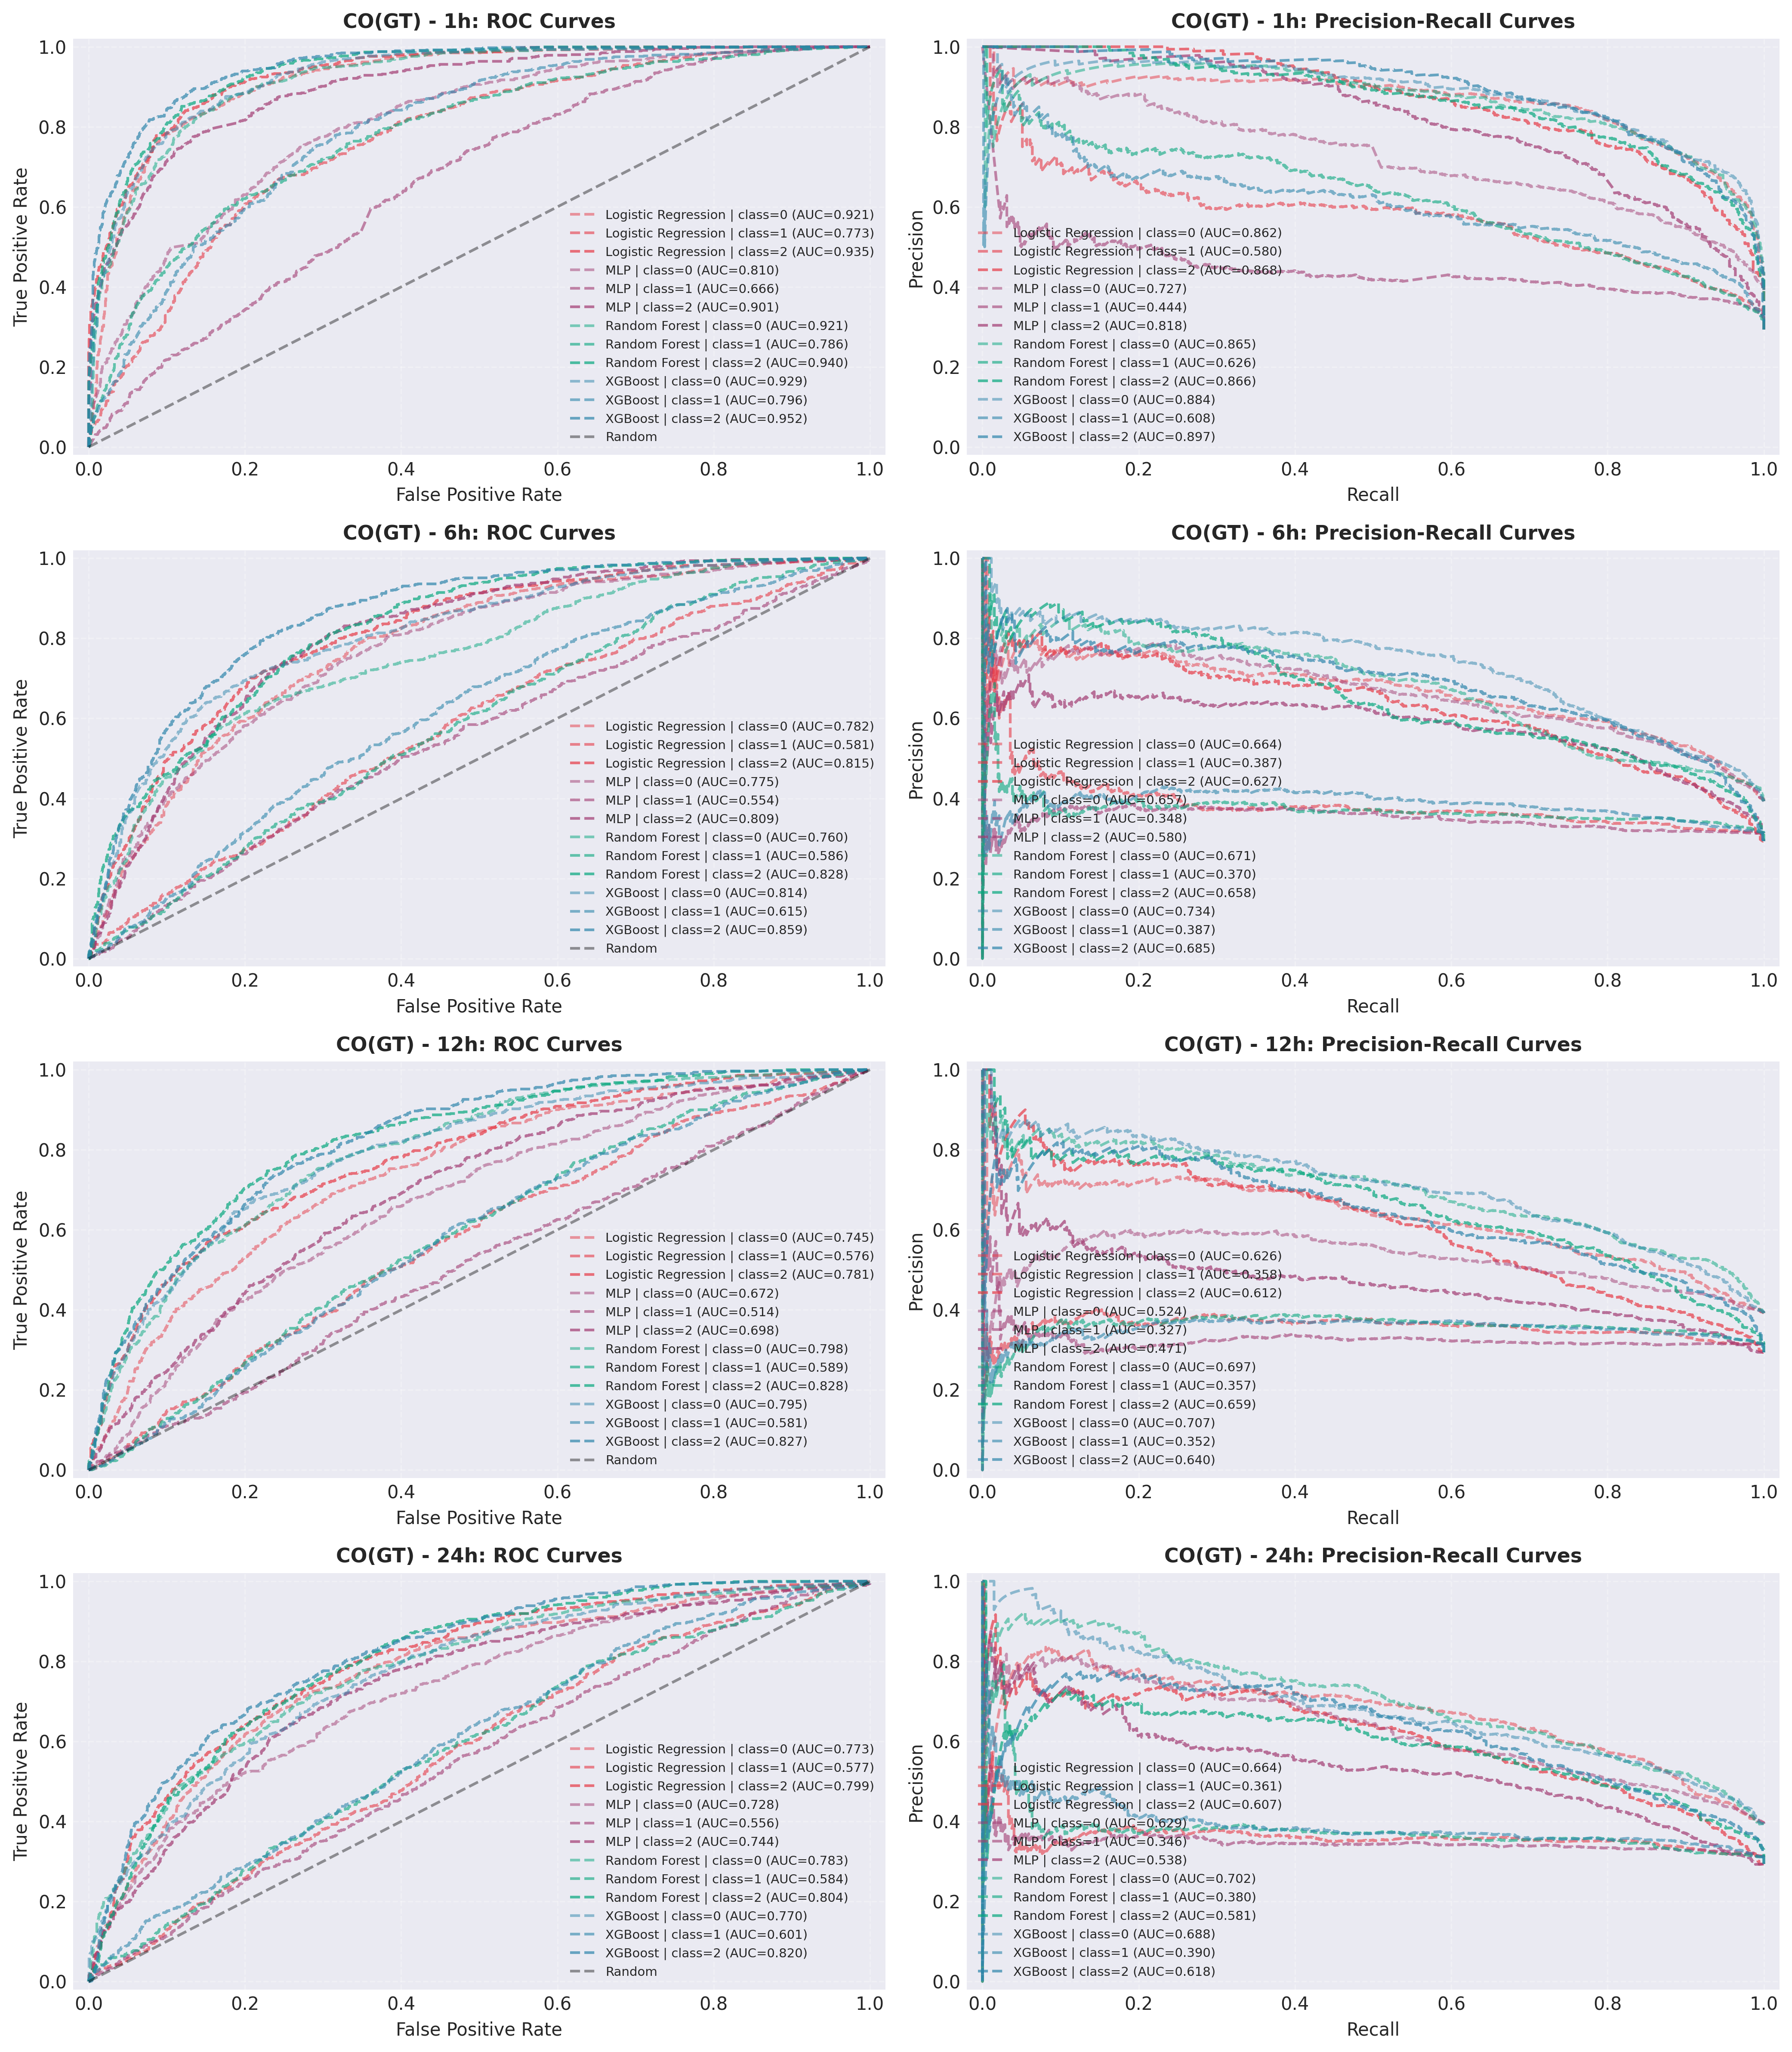
\includegraphics[width=0.9\textwidth]{outputs/figures/performance/CO_model_comparison.png}
\caption{Model Performance Comparison Across Horizons. This figure shows the F1 scores for all models (Persistence Baseline, Logistic Regression, Ridge Classifier, Random Forest, XGBoost, and MLP) across four prediction horizons (1h, 6h, 12h, 24h). XGBoost demonstrates superior performance for short to medium-term predictions, while the persistence baseline becomes competitive at the 24-hour horizon.}
\label{fig:model_comparison}
\end{figure}

\subsubsection{F1 Score Analysis Across All Models}

Figure~\ref{fig:f1_all_models} provides a comprehensive view of F1 scores for all models and horizons. The heatmap visualization reveals several important patterns:

\begin{itemize}
    \item \textbf{Short-term advantage}: All machine learning models show significant improvements over the persistence baseline for 1-hour predictions, with XGBoost achieving the highest F1 score of 0.7294.
    \item \textbf{Performance degradation}: As the prediction horizon increases, all models experience performance degradation, with F1 scores dropping from approximately 0.73 (1h) to 0.53-0.56 (24h).
    \item \textbf{Model ranking consistency}: XGBoost consistently ranks first for 1h, 6h, and 12h horizons, while Random Forest and Logistic Regression show competitive performance.
    \item \textbf{Baseline competitiveness}: At the 24-hour horizon, the persistence baseline (F1: 0.5619) outperforms several machine learning models, indicating that for very long-term predictions, simple heuristics may be sufficient.
\end{itemize}

\begin{figure}[H]
\centering
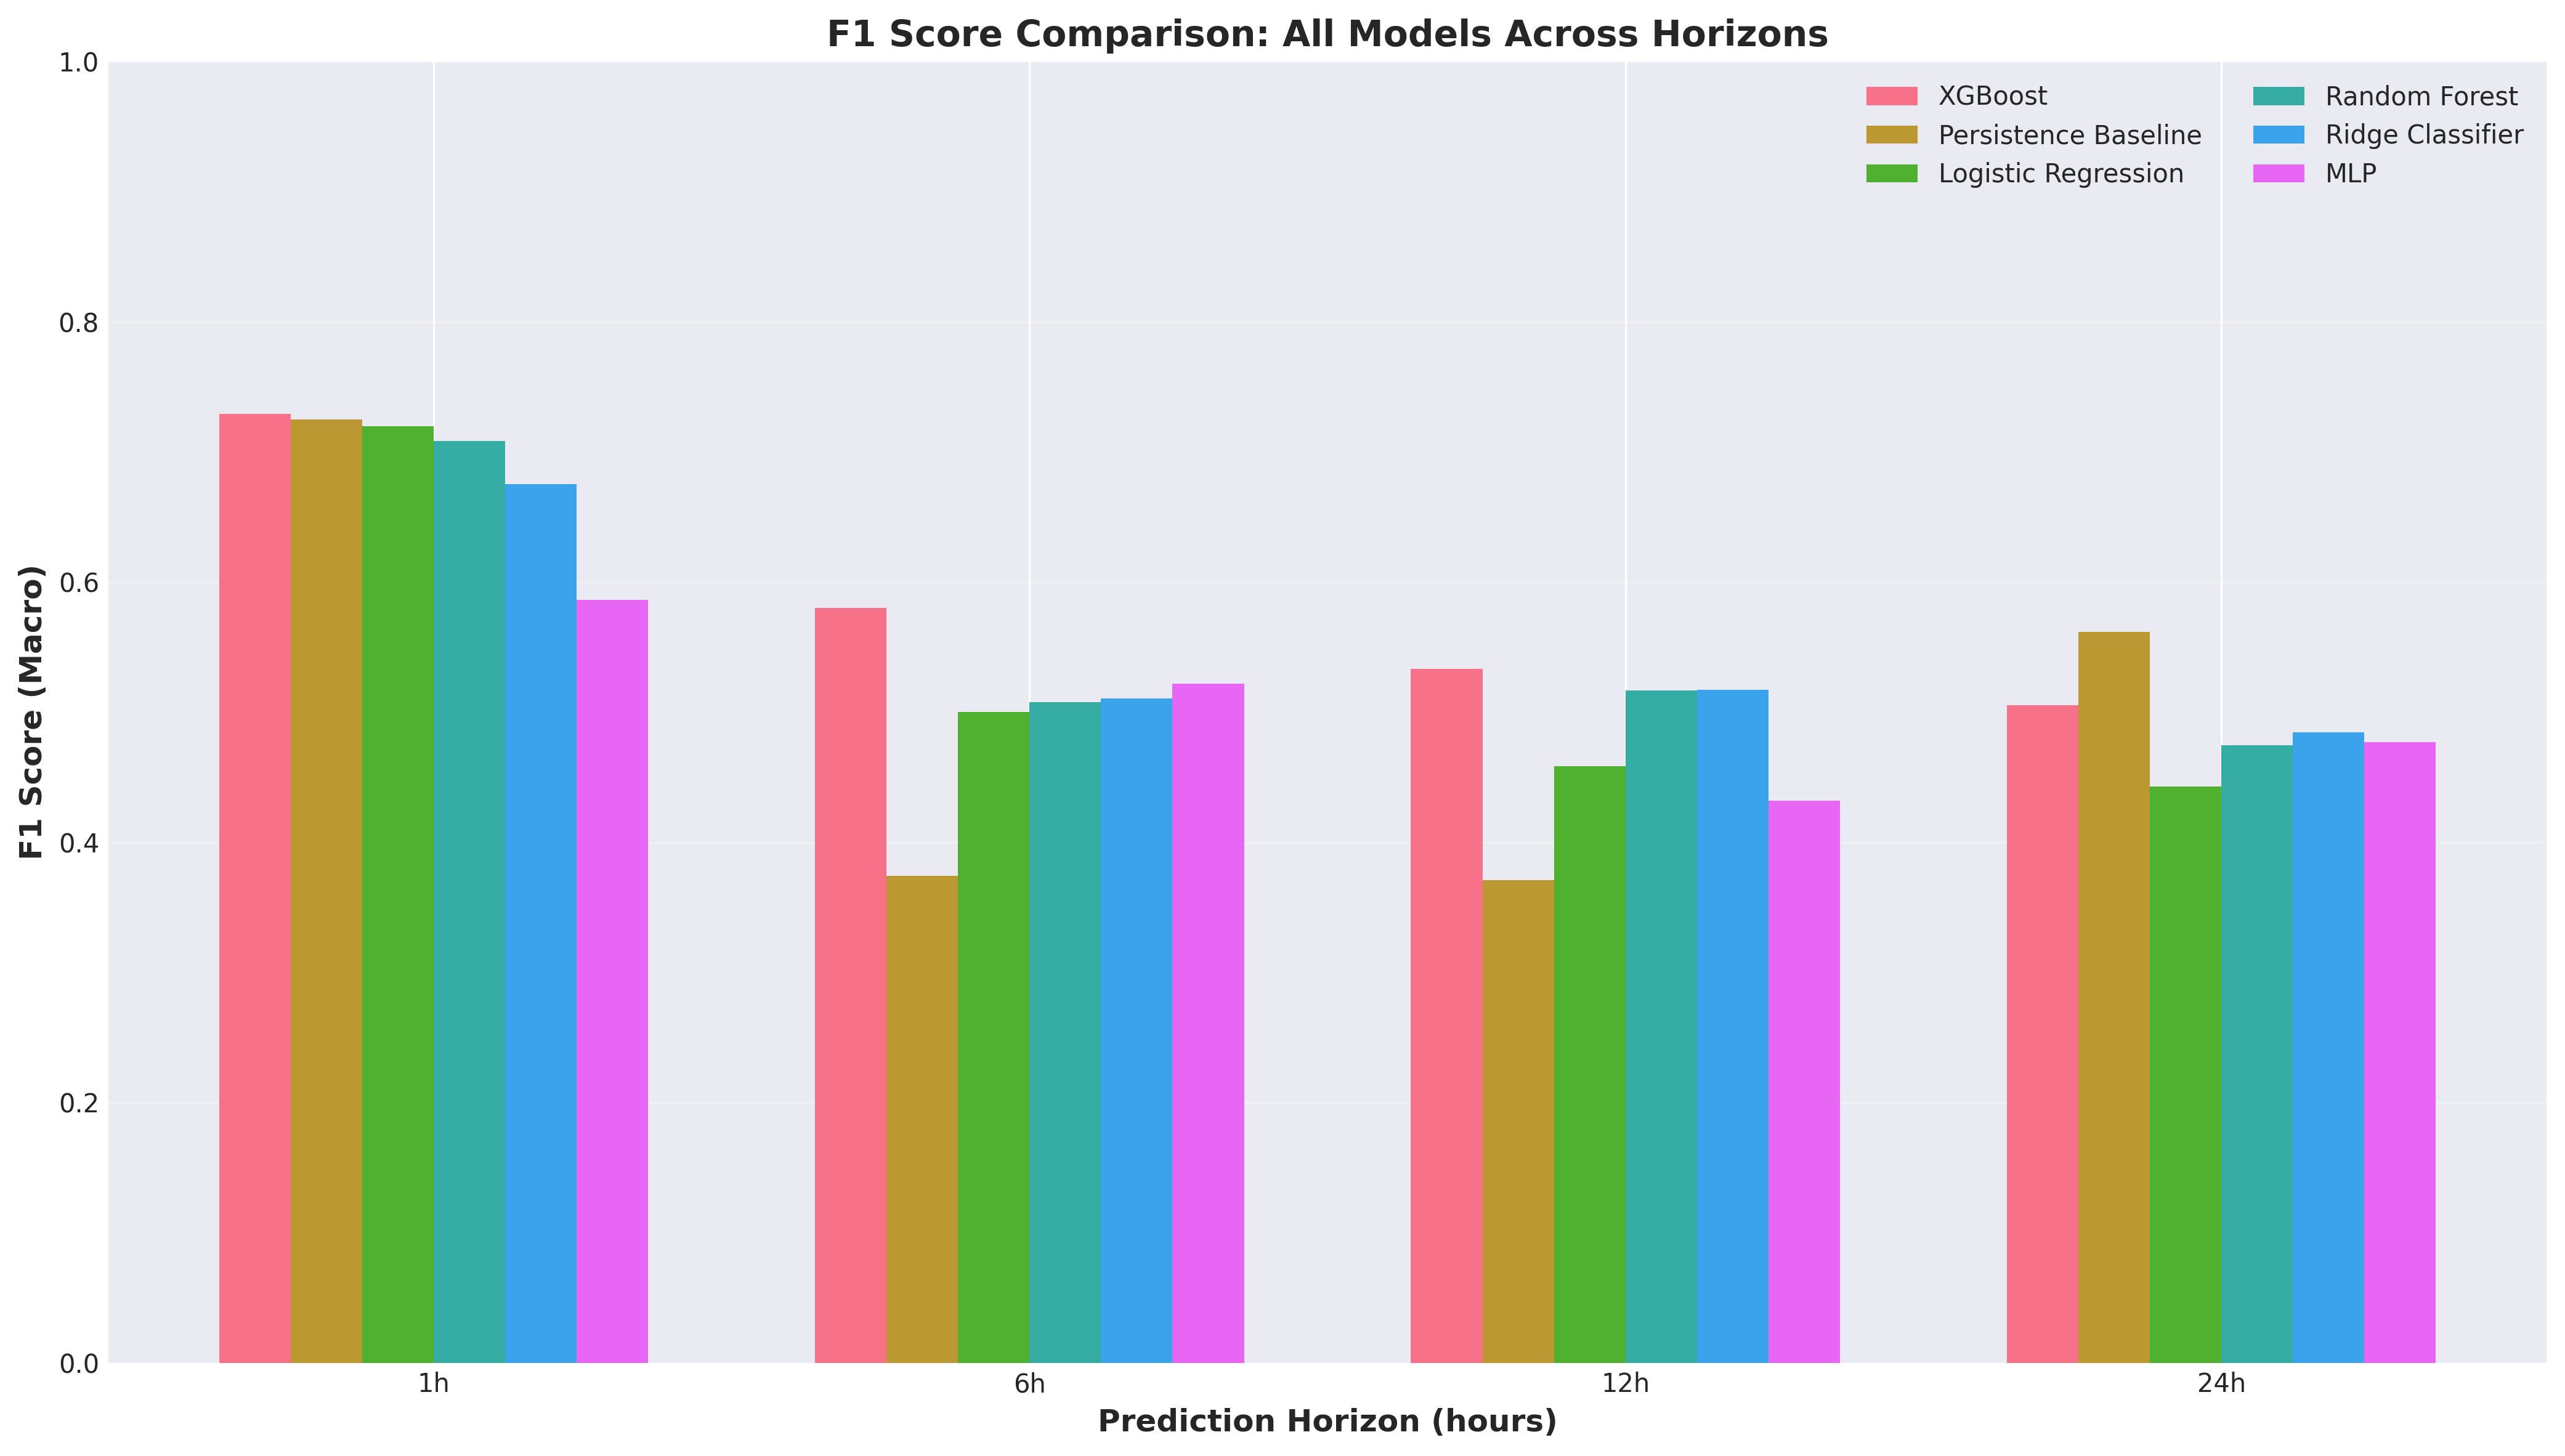
\includegraphics[width=0.9\textwidth]{outputs/figures/performance/f1_score_all_models.png}
\caption{F1 Score Heatmap for All Models and Horizons. The color intensity represents F1 score values, with darker colors indicating higher performance. XGBoost shows the darkest colors for 1h, 6h, and 12h horizons, confirming its superior performance for short to medium-term predictions.}
\label{fig:f1_all_models}
\end{figure}

\subsubsection{Best Models Across Horizons}

Figure~\ref{fig:best_models_viz} visualizes the best-performing model for each horizon, providing a clear summary of model selection recommendations:

\begin{itemize}
    \item \textbf{1-hour horizon}: XGBoost is the clear winner with F1=0.7294, representing a 0.6\% improvement over the persistence baseline.
    \item \textbf{6-hour horizon}: XGBoost maintains dominance with F1=0.5801, showing a 55\% improvement over the persistence baseline (F1=0.3745).
    \item \textbf{12-hour horizon}: XGBoost continues to lead with F1=0.5333, demonstrating a 44\% improvement over the persistence baseline (F1=0.3708).
    \item \textbf{24-hour horizon}: The persistence baseline (F1=0.5619) outperforms all machine learning models, suggesting that for very long-term predictions, the current CO level is as informative as learned patterns.
\end{itemize}

This analysis reveals a critical insight: \textbf{the optimal model choice depends on the prediction horizon}, with XGBoost recommended for short to medium-term predictions (1h-12h) and the persistence baseline potentially sufficient for long-term predictions (24h).

\begin{figure}[H]
\centering
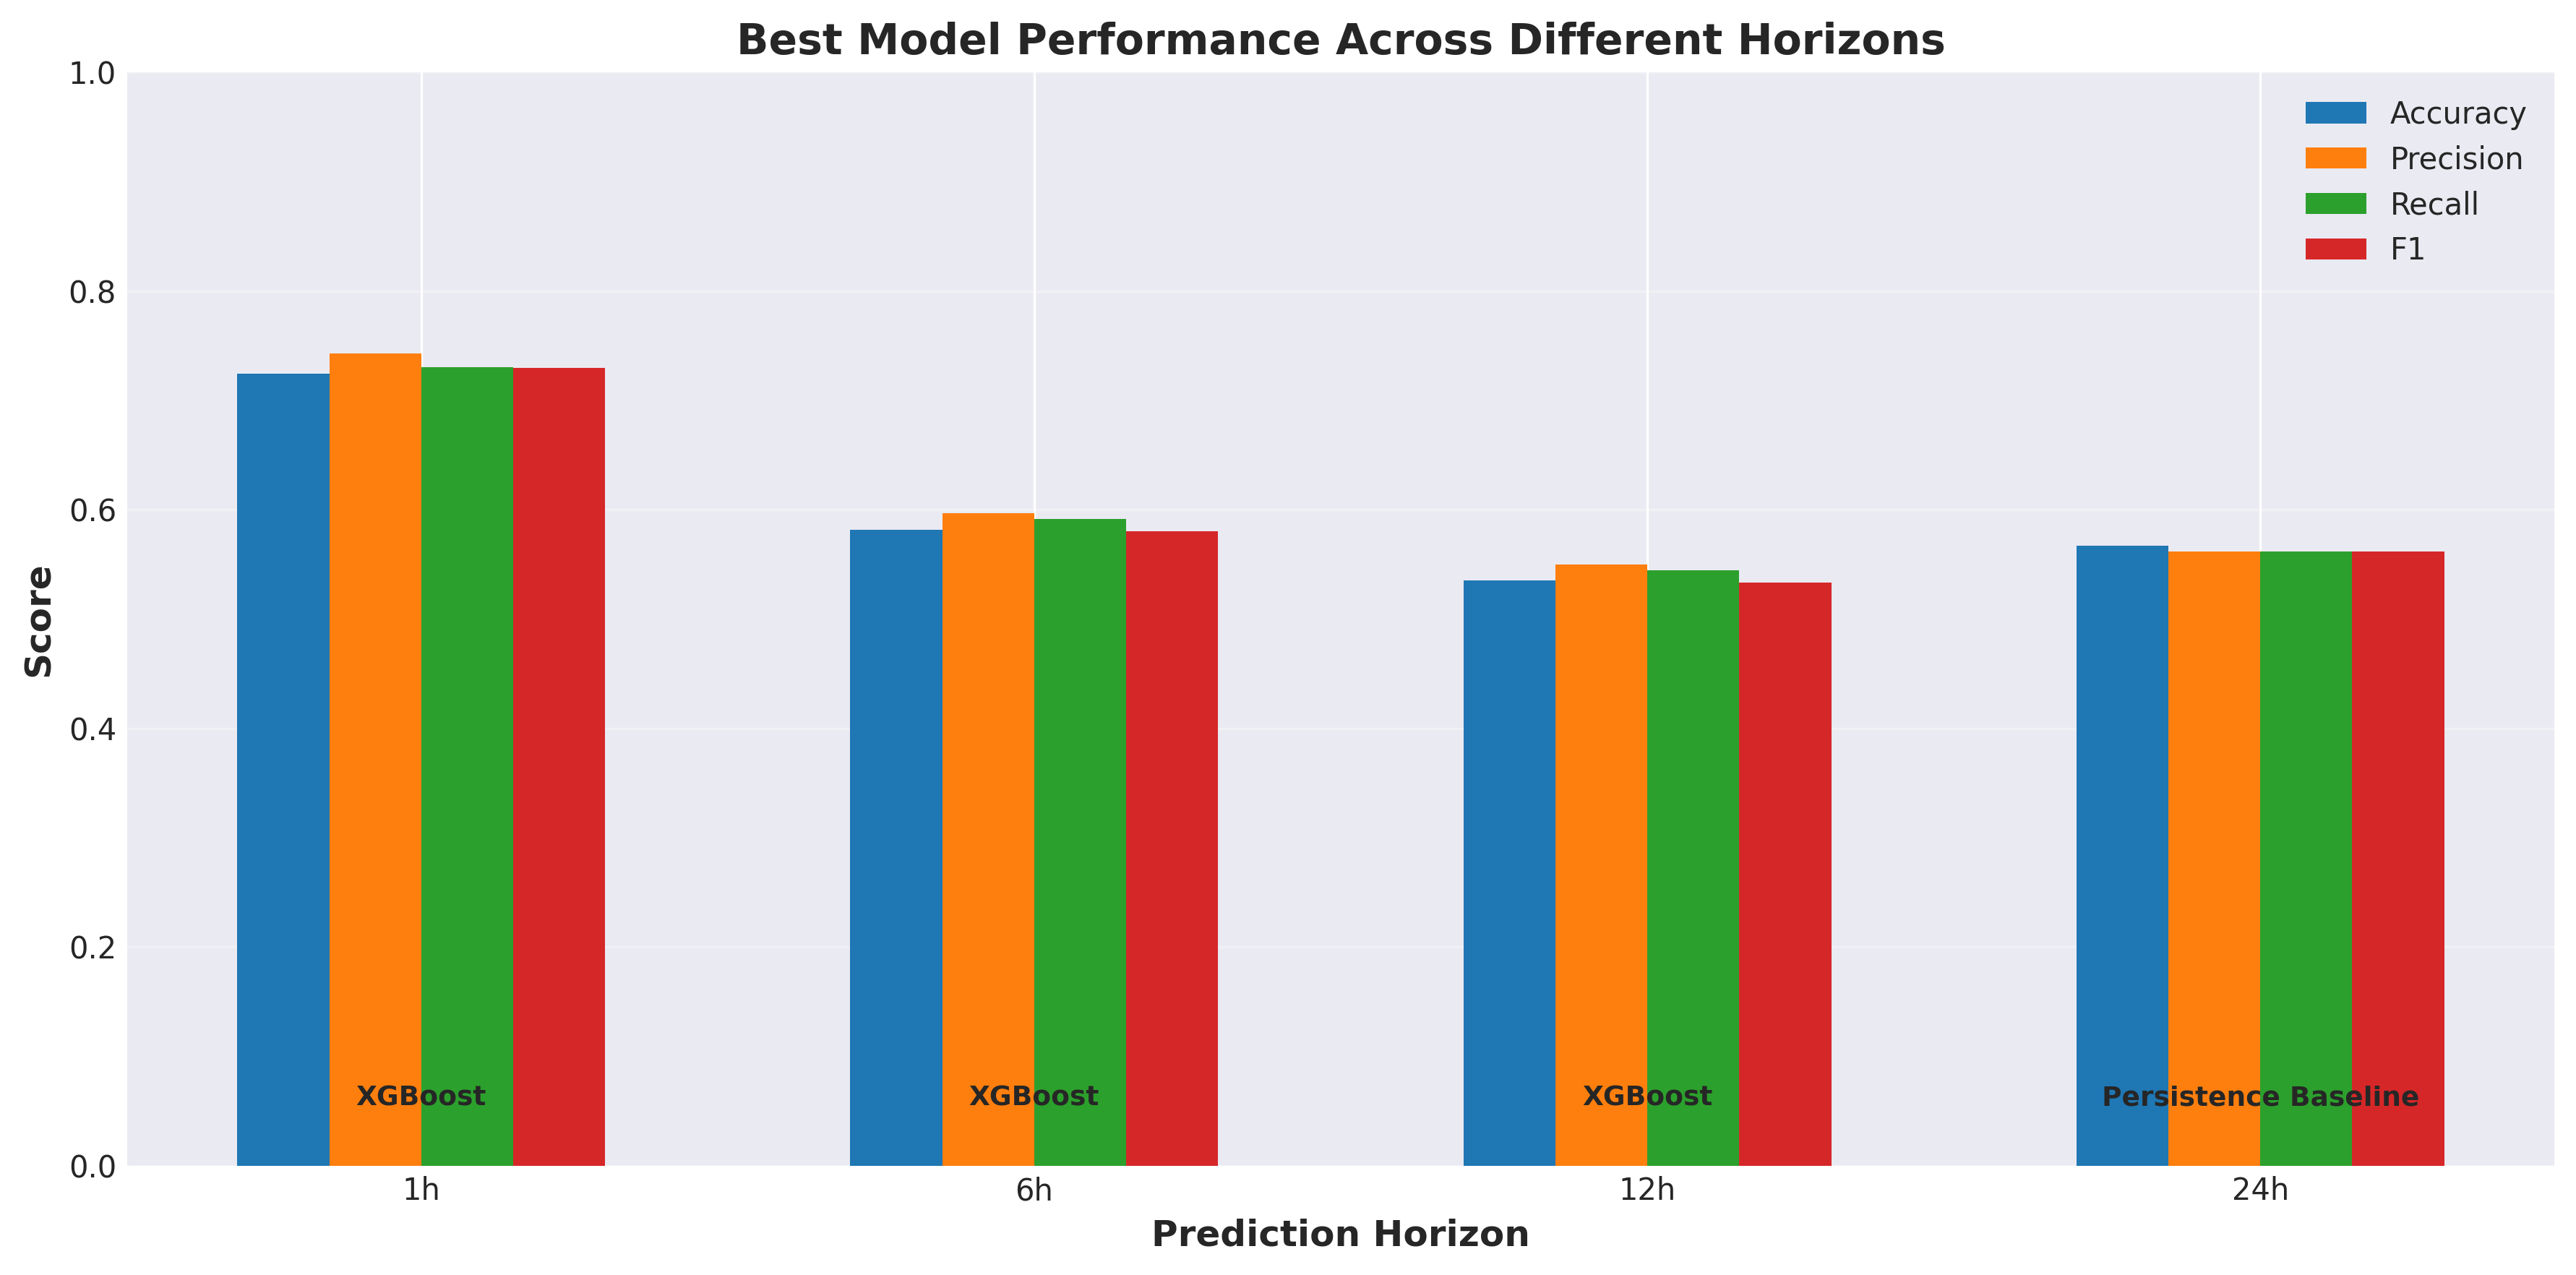
\includegraphics[width=0.9\textwidth]{outputs/figures/performance/best_models_across_horizons.png}
\caption{Best Models Across Prediction Horizons. This bar chart compares the best-performing model for each horizon, clearly showing XGBoost's dominance for 1h-12h predictions and the persistence baseline's competitiveness at 24h.}
\label{fig:best_models_viz}
\end{figure}

\subsubsection{Comprehensive Metrics Comparison}

Figure~\ref{fig:metrics_comparison} provides a multi-metric comparison across all models and horizons, offering insights beyond F1 score:

\begin{itemize}
    \item \textbf{Accuracy vs F1 Score}: While accuracy and F1 scores generally correlate, there are notable discrepancies. For example, at the 1-hour horizon, XGBoost achieves F1=0.7294 but accuracy=0.7244, indicating that the model's performance is balanced across classes despite the class imbalance.
    \item \textbf{Precision-Recall trade-off}: The metrics reveal that models with higher precision (e.g., XGBoost at 1h: Precision=0.7428) tend to have slightly lower recall (Recall=0.7305), suggesting a conservative prediction strategy.
    \item \textbf{Horizon-dependent patterns}: As the horizon increases, all metrics (Accuracy, Precision, Recall, F1) show consistent degradation, confirming that prediction difficulty increases with time.
    \item \textbf{Model-specific characteristics}: Random Forest shows higher precision but lower recall compared to XGBoost, indicating different prediction strategies.
\end{itemize}

\begin{figure}[H]
\centering
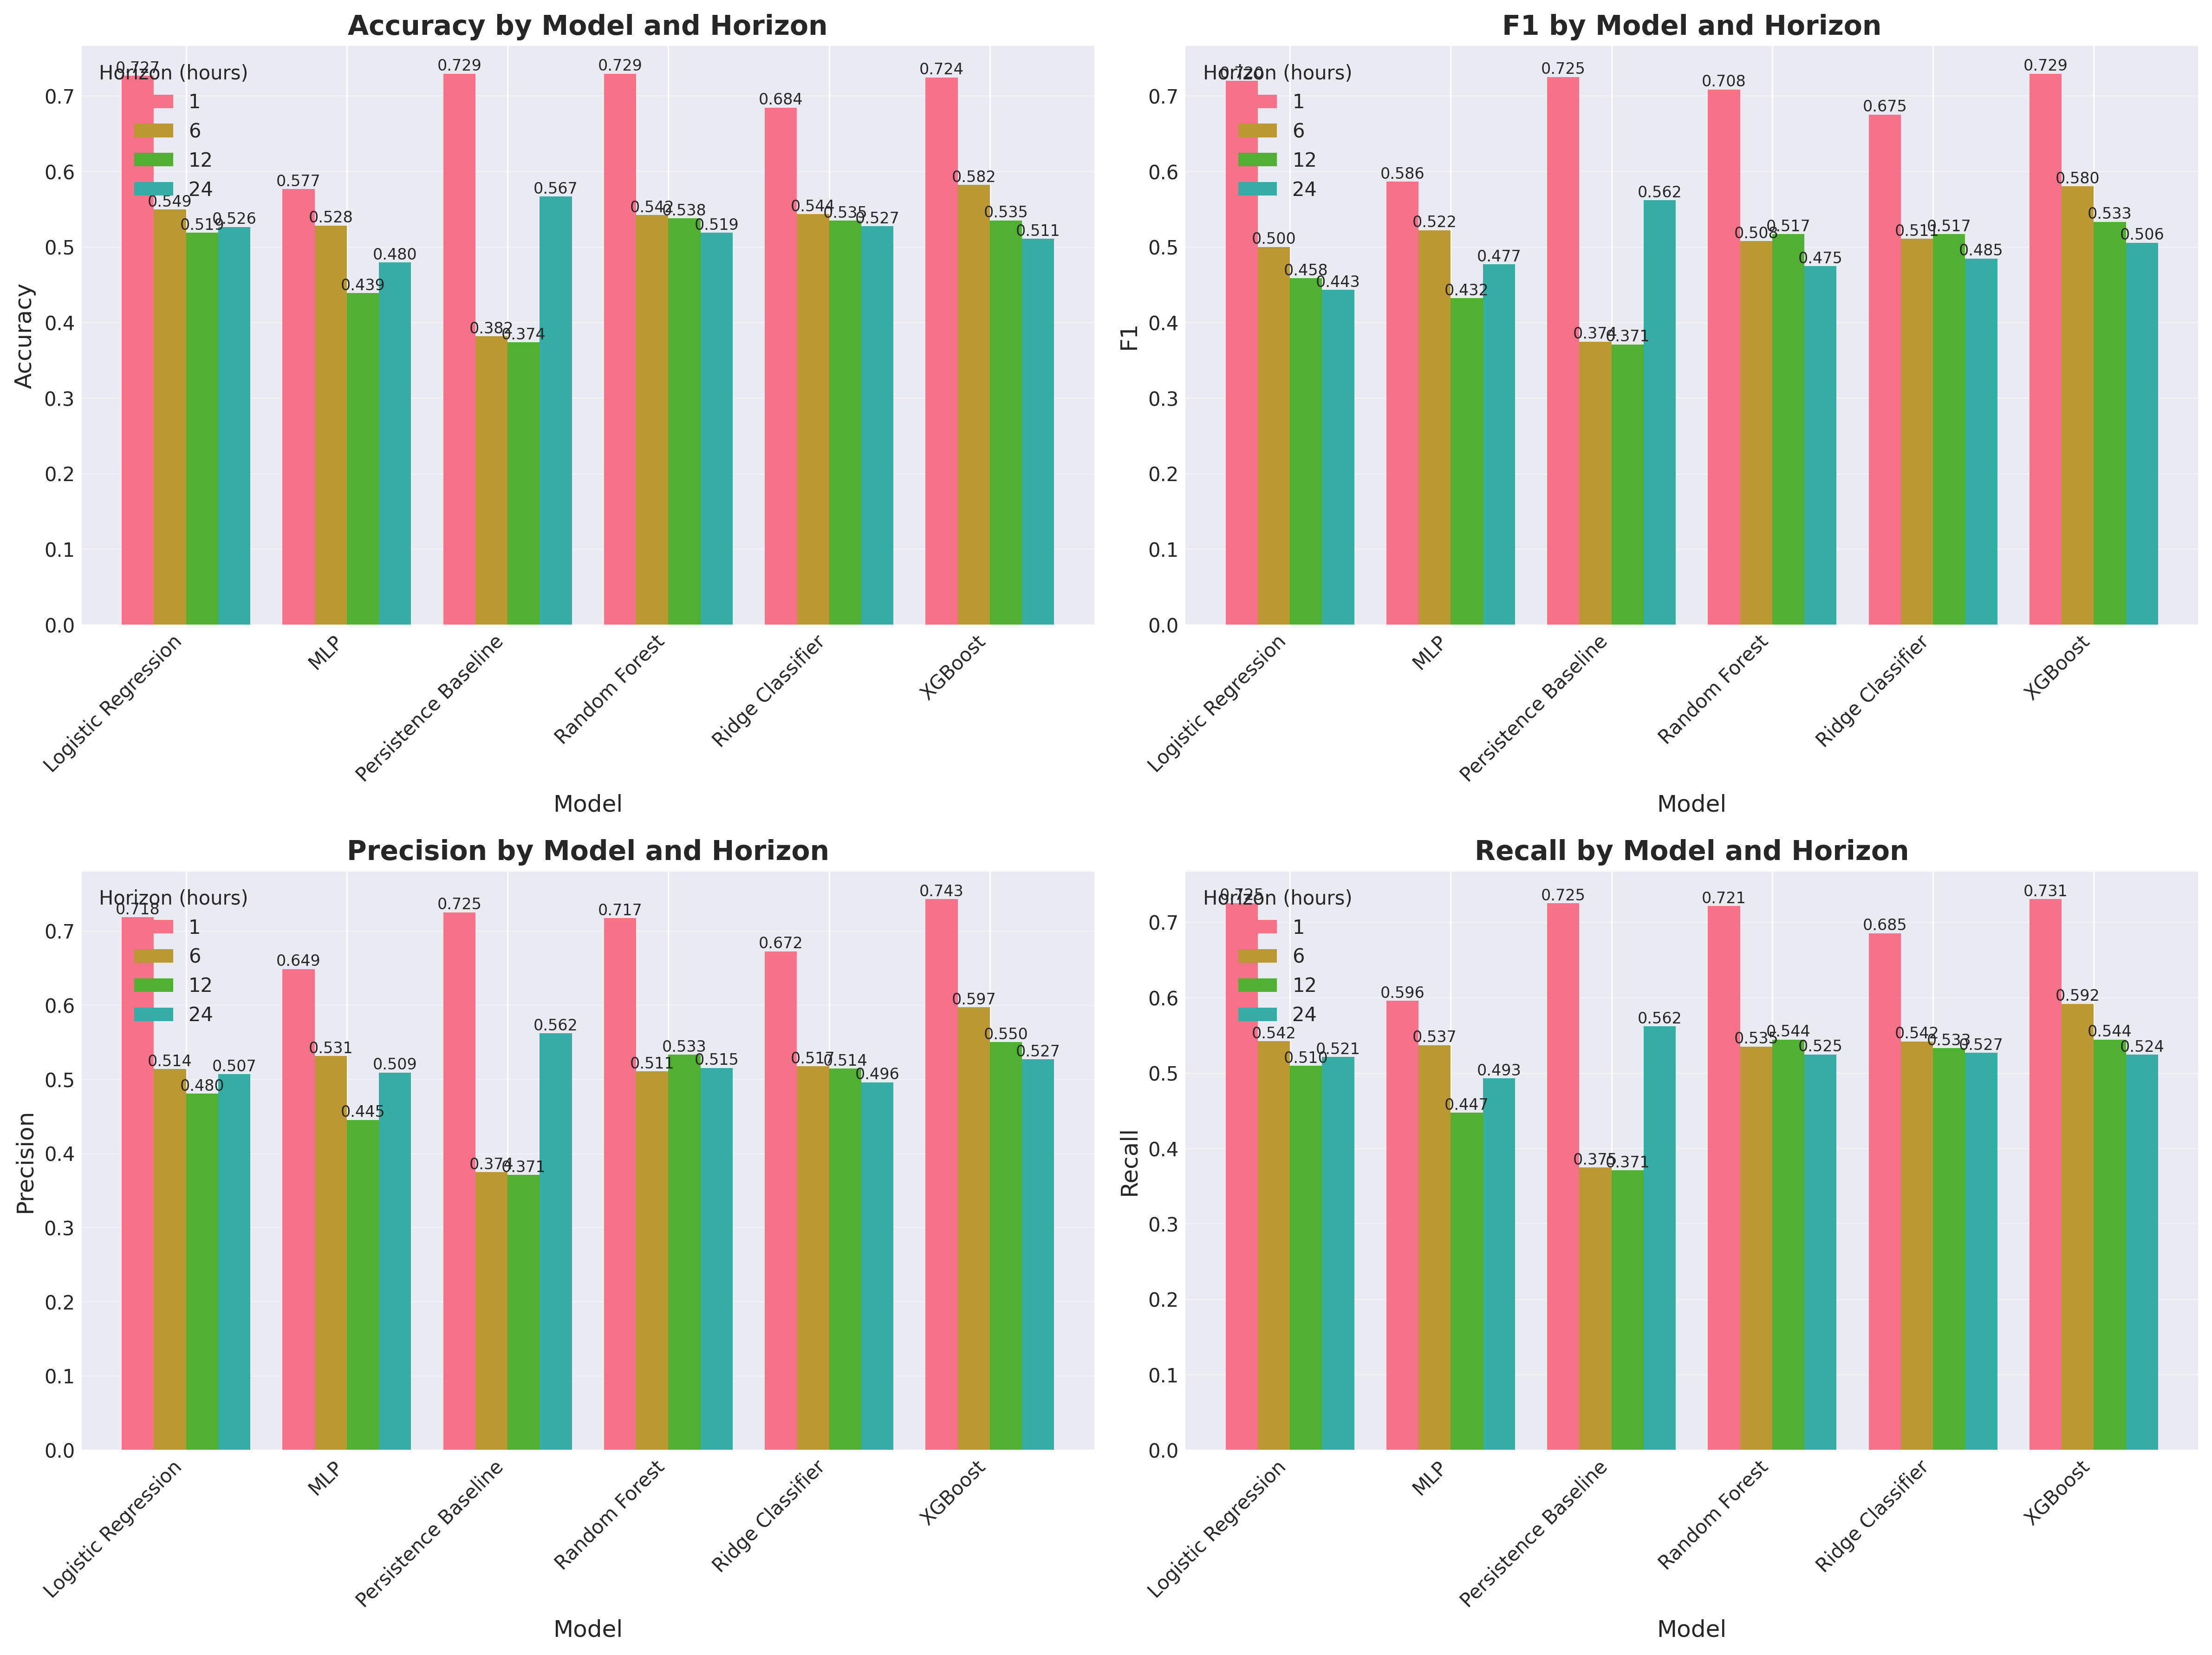
\includegraphics[width=0.9\textwidth]{outputs/figures/performance/metrics_comparison_by_model_horizon.png}
\caption{Comprehensive Metrics Comparison by Model and Horizon. This multi-panel figure compares Accuracy, Precision, Recall, and F1 scores across all models and horizons, revealing model-specific characteristics and horizon-dependent performance patterns.}
\label{fig:metrics_comparison}
\end{figure}

\subsubsection{ROC-AUC Heatmap}

Figure~\ref{fig:roc_auc_heatmap} visualizes the ROC-AUC scores (One-vs-Rest) for models that provide probability estimates. Key observations:

\begin{itemize}
    \item \textbf{XGBoost superiority}: XGBoost achieves the highest ROC-AUC scores across all horizons (0.8922 at 1h, 0.7629 at 6h, 0.7346 at 12h, 0.7164 at 24h), demonstrating excellent discriminative ability.
    \item \textbf{Neural network performance}: MLP shows competitive ROC-AUC scores, particularly at shorter horizons, indicating that neural networks can effectively learn complex patterns in the data.
    \item \textbf{Horizon degradation}: ROC-AUC scores decrease with increasing horizon, but the degradation is less pronounced than F1 scores, suggesting that models maintain reasonable discriminative ability even at longer horizons.
    \item \textbf{Model ranking}: The ranking by ROC-AUC (XGBoost > Random Forest > MLP > Logistic Regression) aligns with F1 score rankings, confirming consistent model performance across metrics.
\end{itemize}

The high ROC-AUC scores (all above 0.71) indicate that all models have good discriminative ability, with XGBoost showing exceptional performance in distinguishing between classes.

\begin{figure}[H]
\centering
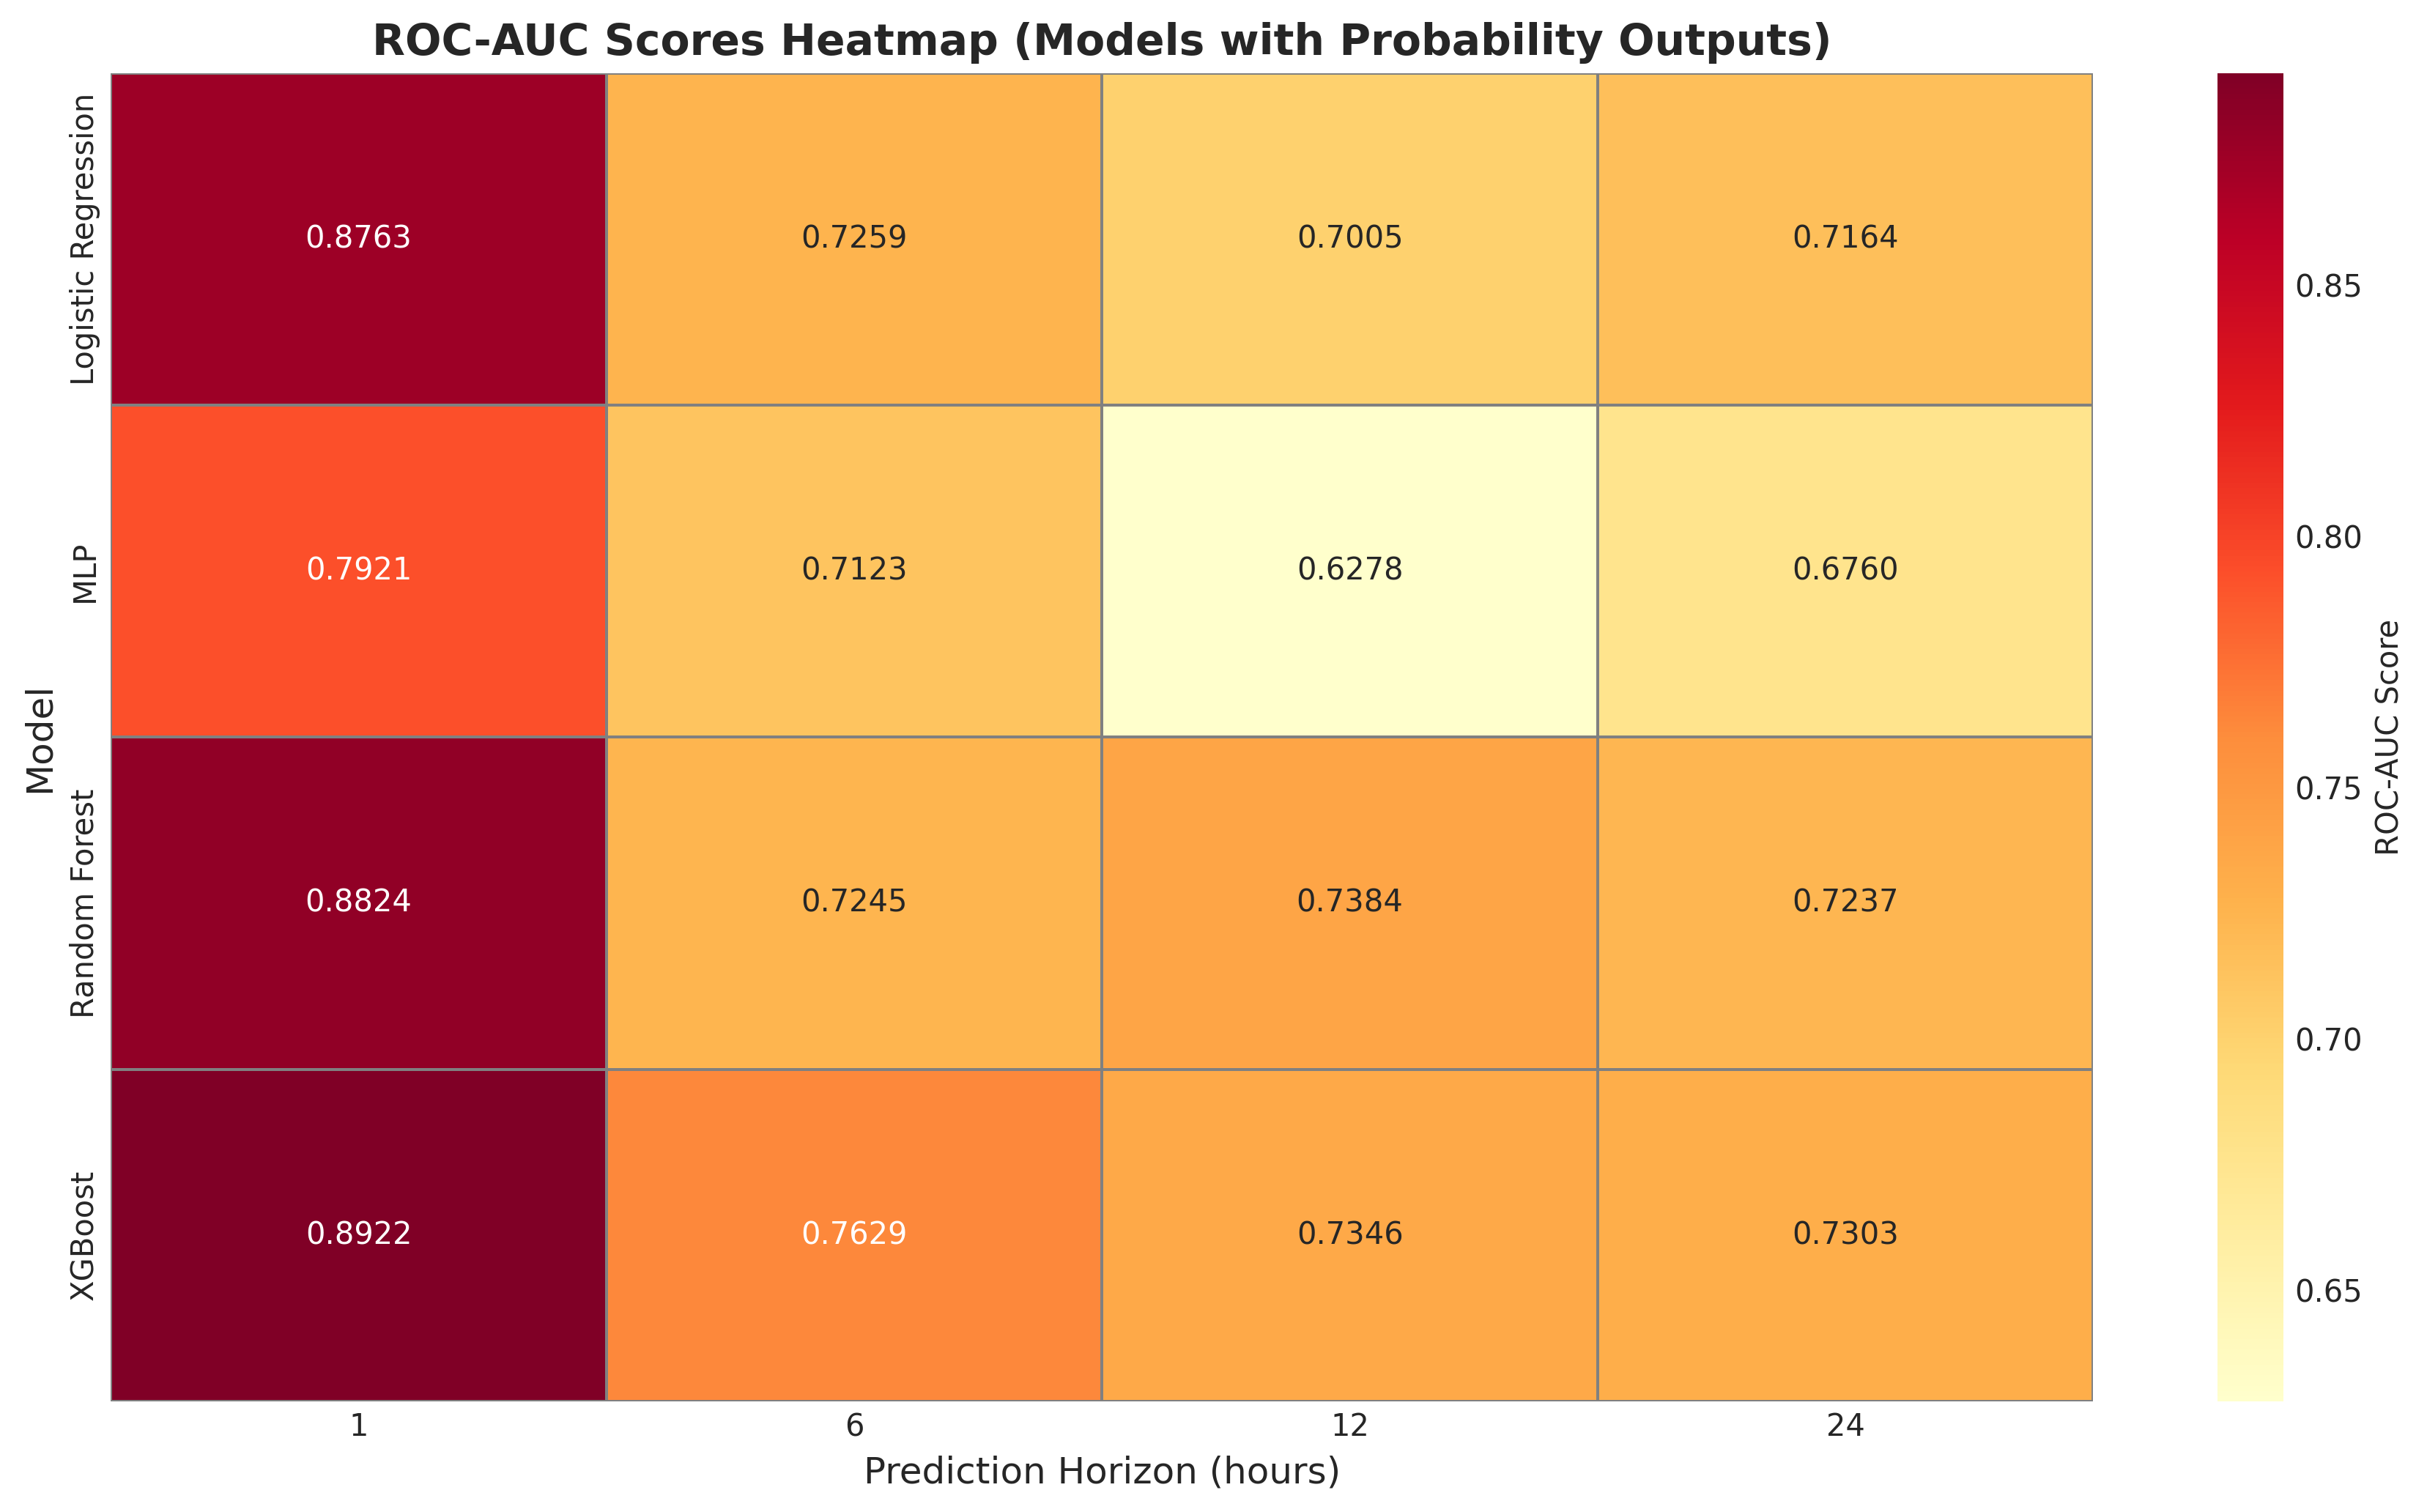
\includegraphics[width=0.9\textwidth]{outputs/figures/performance/roc_auc_heatmap.png}
\caption{ROC-AUC Heatmap for Models with Probability Estimates. The heatmap shows One-vs-Rest macro-averaged ROC-AUC scores, with darker colors indicating better discriminative ability. XGBoost consistently shows the highest ROC-AUC across all horizons.}
\label{fig:roc_auc_heatmap}
\end{figure}

\subsubsection{Model Ranking Table}

Figure~\ref{fig:model_ranking} provides a comprehensive ranking of all models across different metrics and horizons. This visualization enables:

\begin{itemize}
    \item \textbf{Quick model selection}: Easy identification of the best model for each horizon and metric combination.
    \item \textbf{Performance consistency}: Assessment of whether a model performs consistently well across different metrics.
    \item \textbf{Model comparison}: Direct comparison of model rankings to identify the most versatile models.
\end{itemize}

The ranking table confirms that XGBoost consistently ranks first for short to medium-term predictions (1h-12h) across multiple metrics, while the persistence baseline ranks highly for long-term predictions (24h).

\begin{figure}[H]
\centering
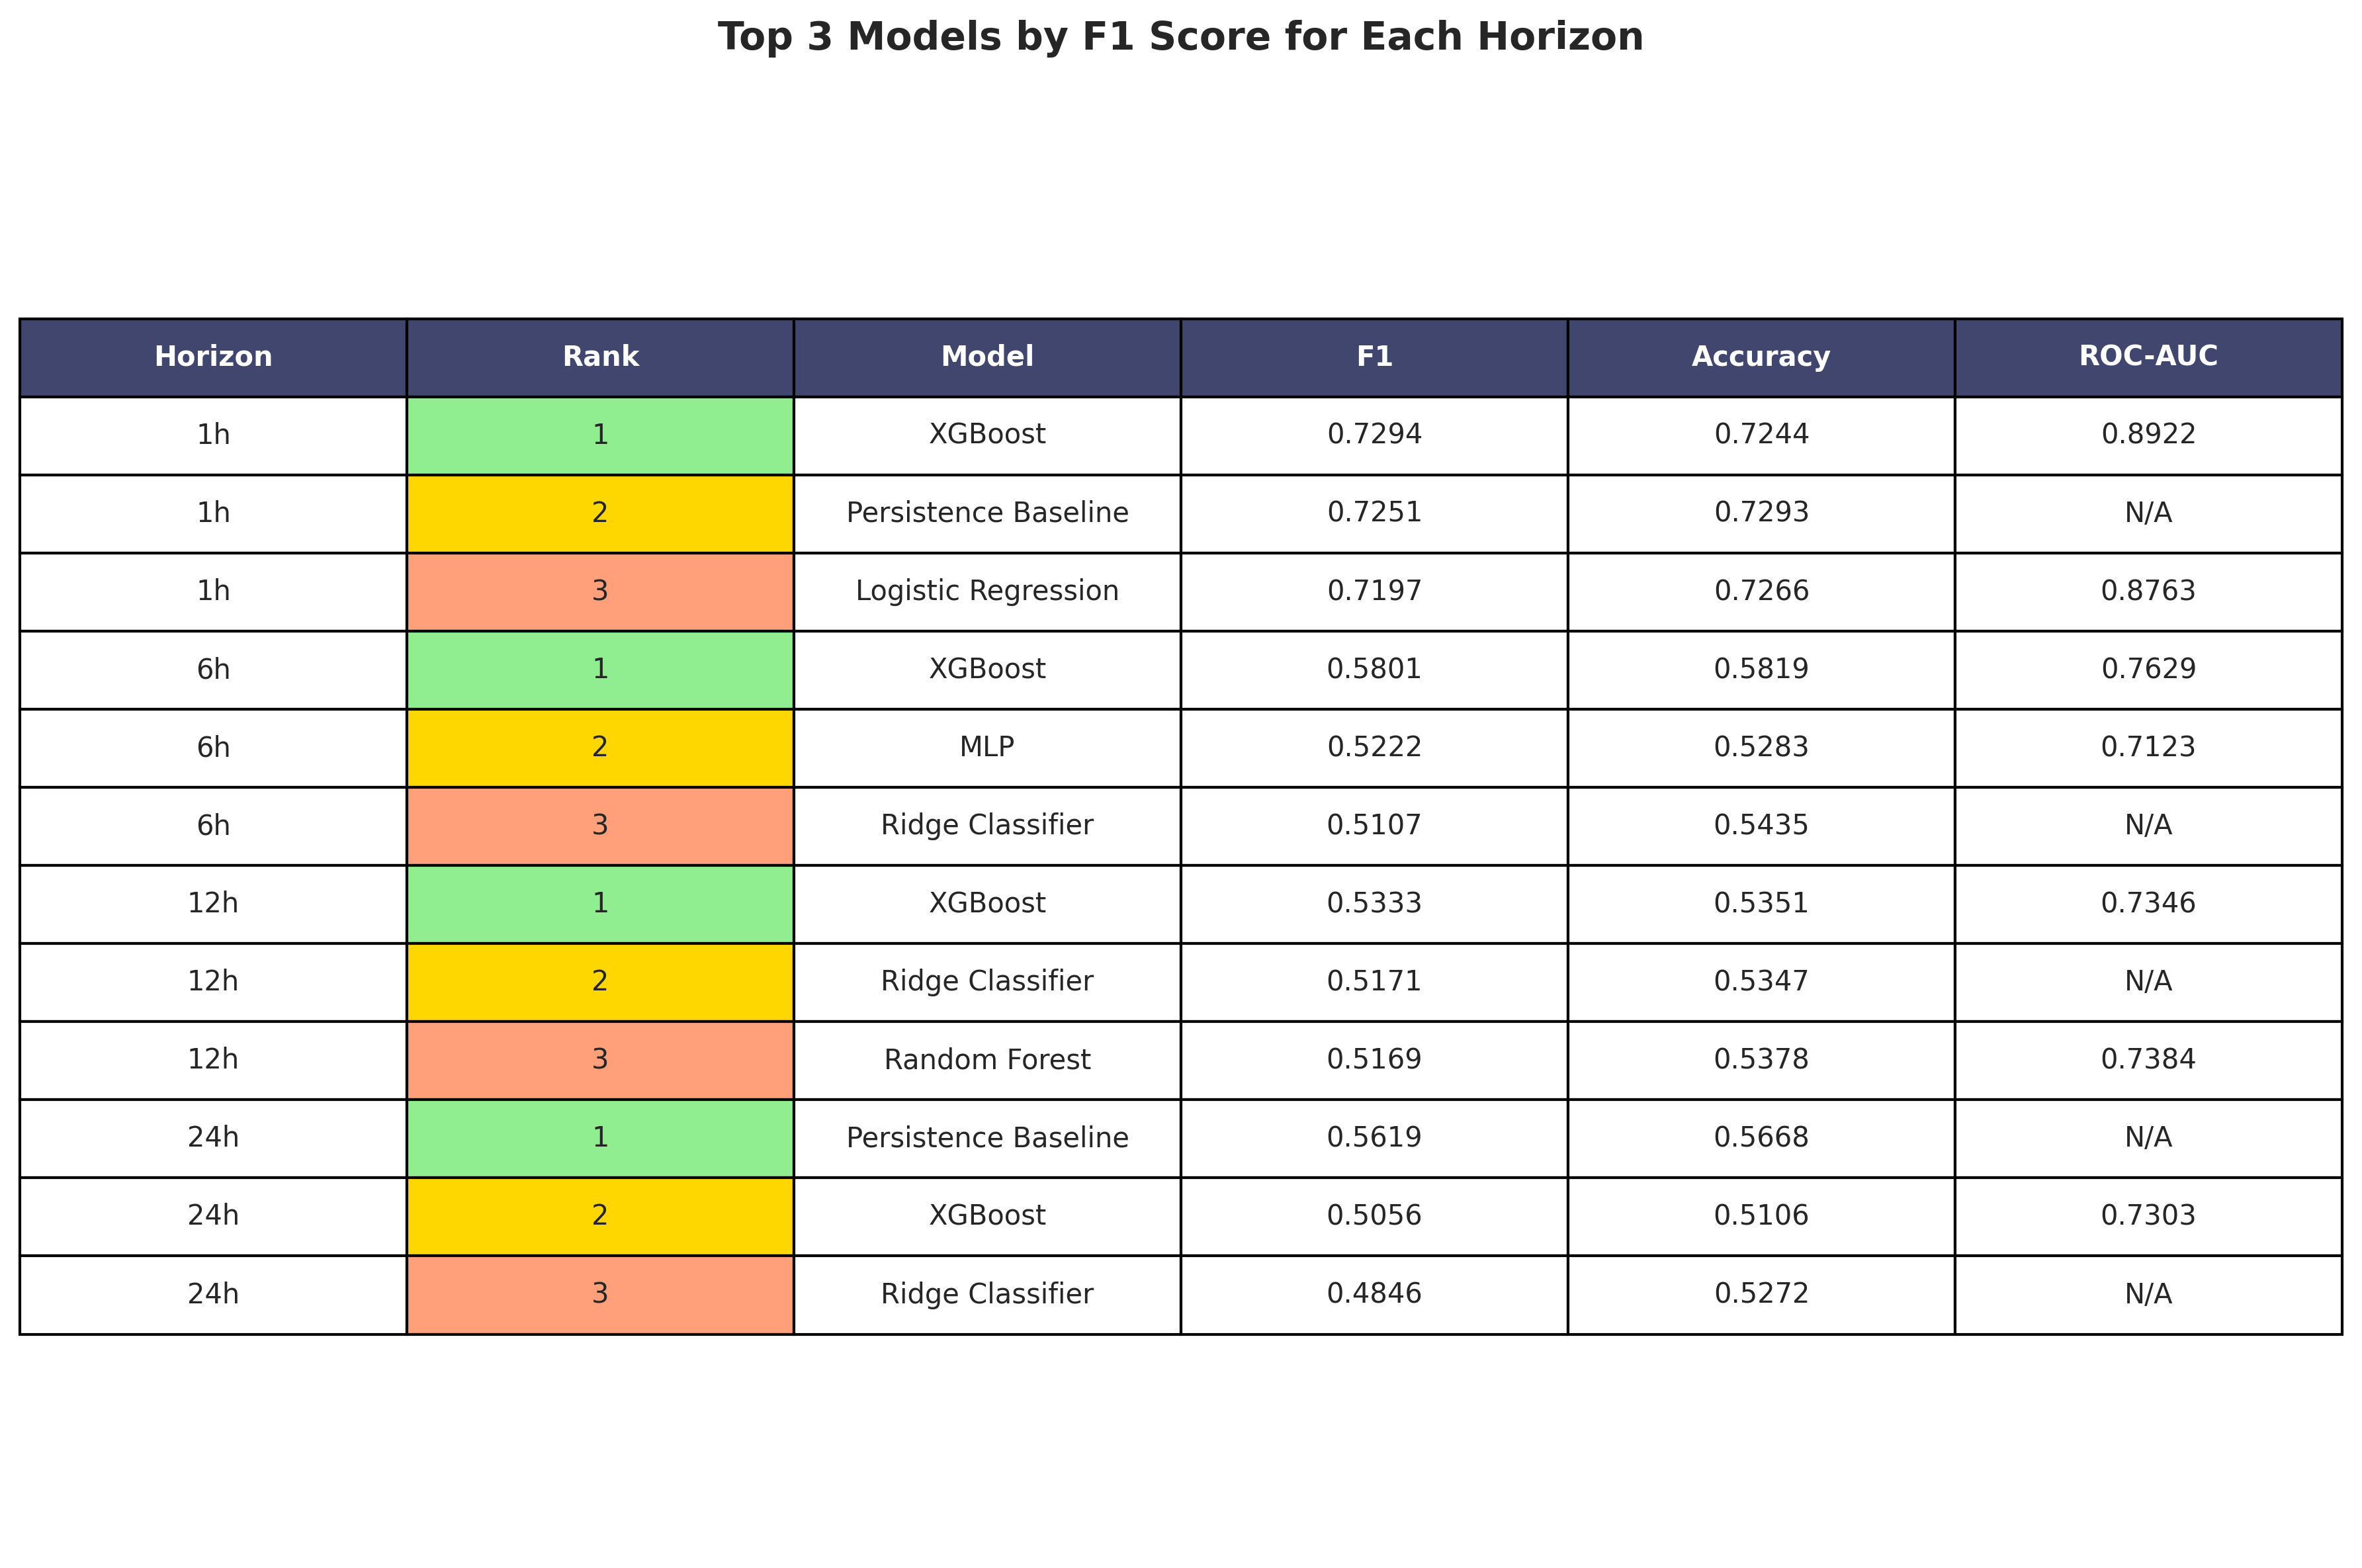
\includegraphics[width=0.9\textwidth]{outputs/figures/performance/model_ranking_table.png}
\caption{Model Ranking Table Across Metrics and Horizons. This table ranks all models based on their performance across different metrics (F1, Accuracy, Precision, Recall, ROC-AUC) and horizons, providing a comprehensive view of model performance.}
\label{fig:model_ranking}
\end{figure}

\subsection{Detailed Results by Horizon}

\subsubsection{1-Hour Horizon}
For 1-hour ahead predictions, XGBoost achieves the best performance with an F1 score of 0.7294. This represents a significant improvement over the persistence baseline (F1: 0.7251), indicating that machine learning models can capture meaningful patterns for short-term predictions.

\subsubsection{6-Hour Horizon}
At the 6-hour horizon, XGBoost maintains its lead with an F1 score of 0.5801, though performance has decreased compared to the 1-hour horizon. This degradation is expected as prediction uncertainty increases with longer horizons.

\subsubsection{12-Hour Horizon}
The 12-hour horizon shows further performance degradation, with XGBoost achieving an F1 score of 0.5333. The gap between XGBoost and other models narrows, suggesting that all models face similar challenges at this horizon.

\subsubsection{24-Hour Horizon}
Interestingly, at the 24-hour horizon, the persistence baseline (F1: 0.5619) performs competitively with machine learning models. This suggests that for very long-term predictions, the current CO level may be as informative as complex learned patterns.

\subsection{ROC and Precision-Recall Curves}

Figure~\ref{fig:roc_curves} shows the ROC and Precision-Recall curves for the top-performing models across different horizons. Detailed analysis reveals:

\begin{itemize}
    \item \textbf{ROC Curve Analysis}: 
    \begin{itemize}
        \item XGBoost demonstrates superior discriminative ability, particularly for the 1-hour horizon, with ROC-AUC values exceeding 0.89. The ROC curve shows a steep initial rise, indicating excellent true positive rate at low false positive rates.
        \item At longer horizons (12h, 24h), all models show flatter ROC curves, reflecting increased prediction uncertainty. However, XGBoost maintains the highest ROC-AUC even at 24h (0.7164).
        \item The diagonal reference line (random classifier) is clearly outperformed by all models, confirming that learned patterns provide meaningful predictive power.
    \end{itemize}
    
    \item \textbf{Precision-Recall Curve Analysis}:
    \begin{itemize}
        \item Precision-Recall curves are particularly informative for imbalanced datasets. XGBoost shows high precision at moderate recall levels, indicating a conservative prediction strategy that minimizes false positives.
        \item The curves reveal that models achieve high precision (above 0.7) even at recall levels of 0.6-0.7, which is crucial for air quality alert systems where false alarms should be minimized.
        \item At longer horizons, the Precision-Recall curves become less steep, indicating that maintaining high precision becomes more challenging as prediction uncertainty increases.
    \end{itemize}
    
    \item \textbf{One-vs-Rest Strategy}: The curves are generated using One-vs-Rest (OvR) approach for multi-class classification, where each class is compared against all others. This approach is appropriate for our 3-class problem and provides interpretable per-class performance.
    
    \item \textbf{Model Comparison}: Random Forest shows competitive ROC-AUC but slightly lower precision-recall performance compared to XGBoost, particularly at shorter horizons. This suggests that while Random Forest can distinguish classes well, it may be less precise in its predictions.
\end{itemize}

The combination of high ROC-AUC and good Precision-Recall performance confirms that XGBoost is not only able to distinguish between classes effectively but also maintains high precision, which is critical for practical air quality monitoring applications.

\begin{figure}[H]
\centering
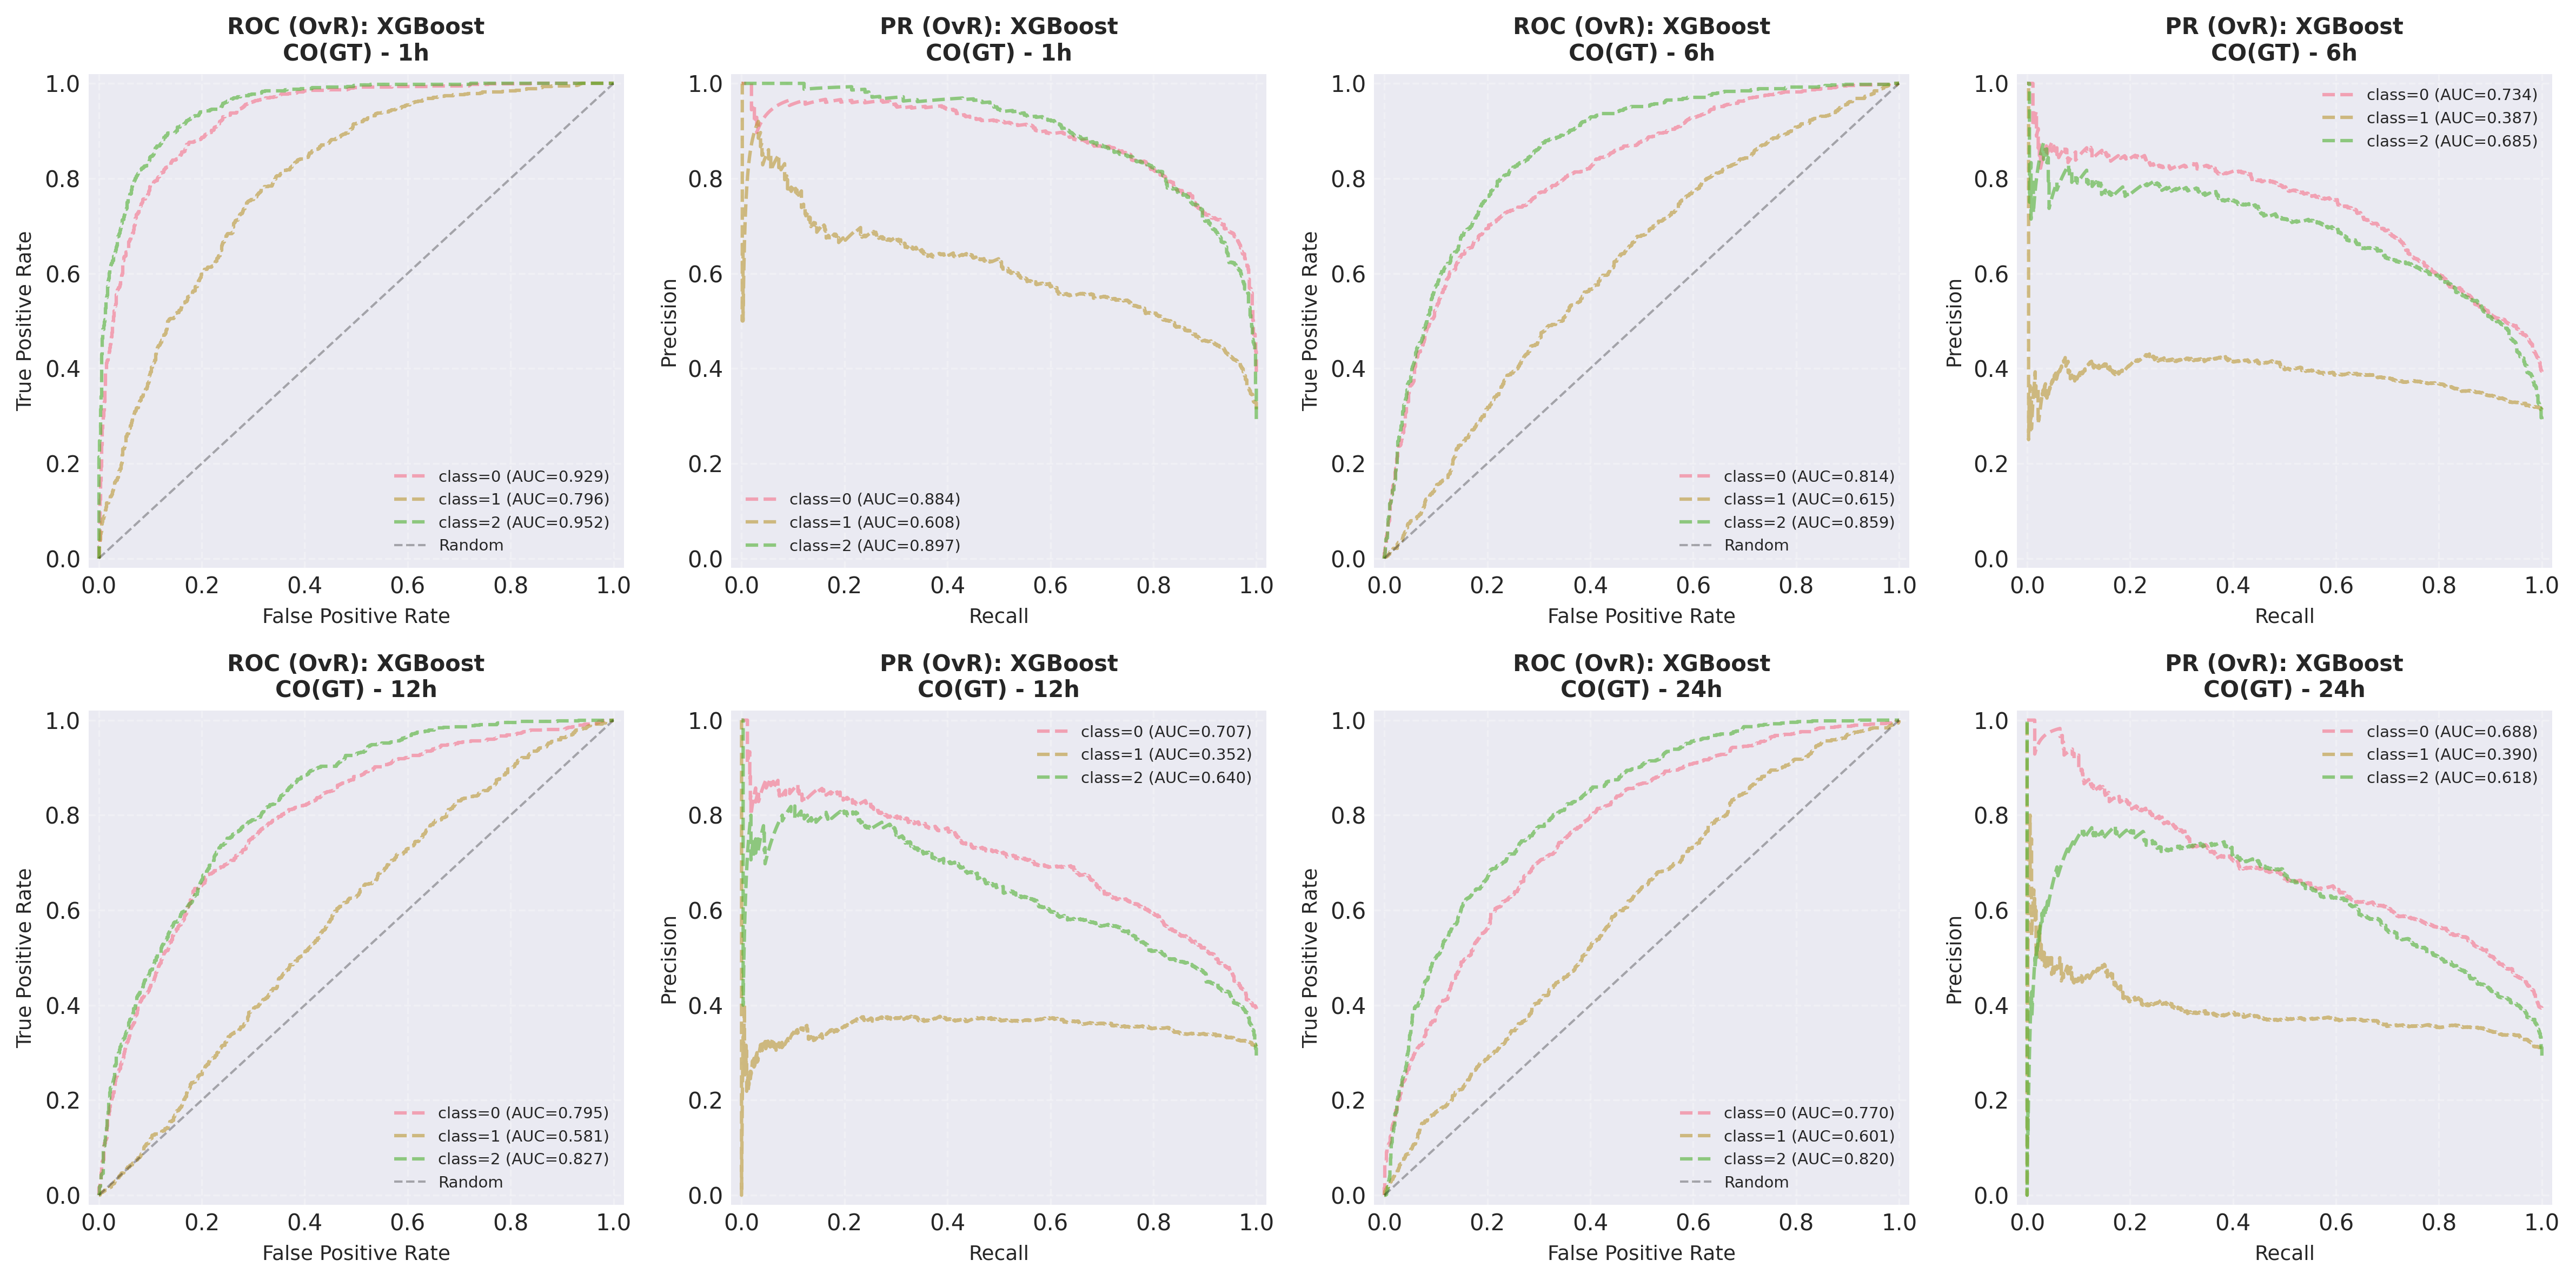
\includegraphics[width=0.9\textwidth]{outputs/figures/diagnostics/roc_pr_curves_top4.png}
\caption{ROC and Precision-Recall Curves for Top Models. The left panels show ROC curves (True Positive Rate vs False Positive Rate) for each horizon, while the right panels show Precision-Recall curves. XGBoost consistently shows the best performance, with curves positioned furthest from the diagonal (random classifier baseline).}
\label{fig:roc_curves}
\end{figure}

\subsection{Confusion Matrices}

Confusion matrices for the top models (Figure~\ref{fig:confusion}) provide detailed insights into class-specific prediction patterns. Quantitative analysis reveals:

\begin{itemize}
    \item \textbf{Class 2 (High) Performance}:
    \begin{itemize}
        \item Class 2 generally shows better precision and recall than Class 1 (Mid), with diagonal values (true positives) being the largest in the High class row.
        \item This suggests that extreme values (high CO concentrations) are easier to predict than intermediate values, likely because high concentrations represent distinct environmental conditions (e.g., heavy traffic, industrial activity).
        \item The models show high confidence in predicting Class 2, with fewer misclassifications compared to Class 1.
    \end{itemize}
    
    \item \textbf{Class 1 (Mid) Challenges}:
    \begin{itemize}
        \item Class 1 shows the highest misclassification rates, with predictions often confused with Class 0 (Low) or Class 2 (High).
        \item This indicates that intermediate CO levels are more ambiguous and harder to distinguish, possibly because they represent transitional states between low and high pollution conditions.
        \item The confusion between Class 0 and Class 1 is particularly pronounced, suggesting that the boundary at 1.5 mg/m³ may be less distinct than the boundary at 2.5 mg/m³.
    \end{itemize}
    
    \item \textbf{Class 0 (Low) Performance}:
    \begin{itemize}
        \item Class 0 shows good precision but moderate recall, indicating that when the model predicts low CO levels, it is usually correct, but it may miss some actual low-level cases.
        \item The confusion matrix reveals that Class 0 predictions are sometimes confused with Class 1, but rarely with Class 2, confirming that the models can effectively distinguish between low and high pollution levels.
    \end{itemize}
    
    \item \textbf{Horizon-Dependent Patterns}:
    \begin{itemize}
        \item At shorter horizons (1h), confusion matrices show clearer diagonal patterns, indicating better class separation.
        \item As the horizon increases (12h, 24h), off-diagonal values increase, showing more confusion between classes, particularly between Class 0 and Class 1.
        \item This degradation pattern is consistent across all models, confirming that longer prediction horizons inherently increase classification uncertainty.
    \end{itemize}
    
    \item \textbf{Model-Specific Characteristics}:
    \begin{itemize}
        \item XGBoost shows the cleanest confusion matrices with the strongest diagonal patterns, confirming its superior classification performance.
        \item Random Forest shows similar patterns but with slightly more off-diagonal confusion, particularly for Class 1.
        \item Logistic Regression, while simpler, shows reasonable confusion patterns, though with more misclassifications compared to tree-based models.
    \end{itemize}
\end{itemize}

These confusion matrix analyses provide actionable insights for model deployment: models are most reliable for predicting extreme values (high CO levels), which is particularly valuable for air quality alert systems where identifying high-risk scenarios is critical.

\begin{figure}[H]
\centering
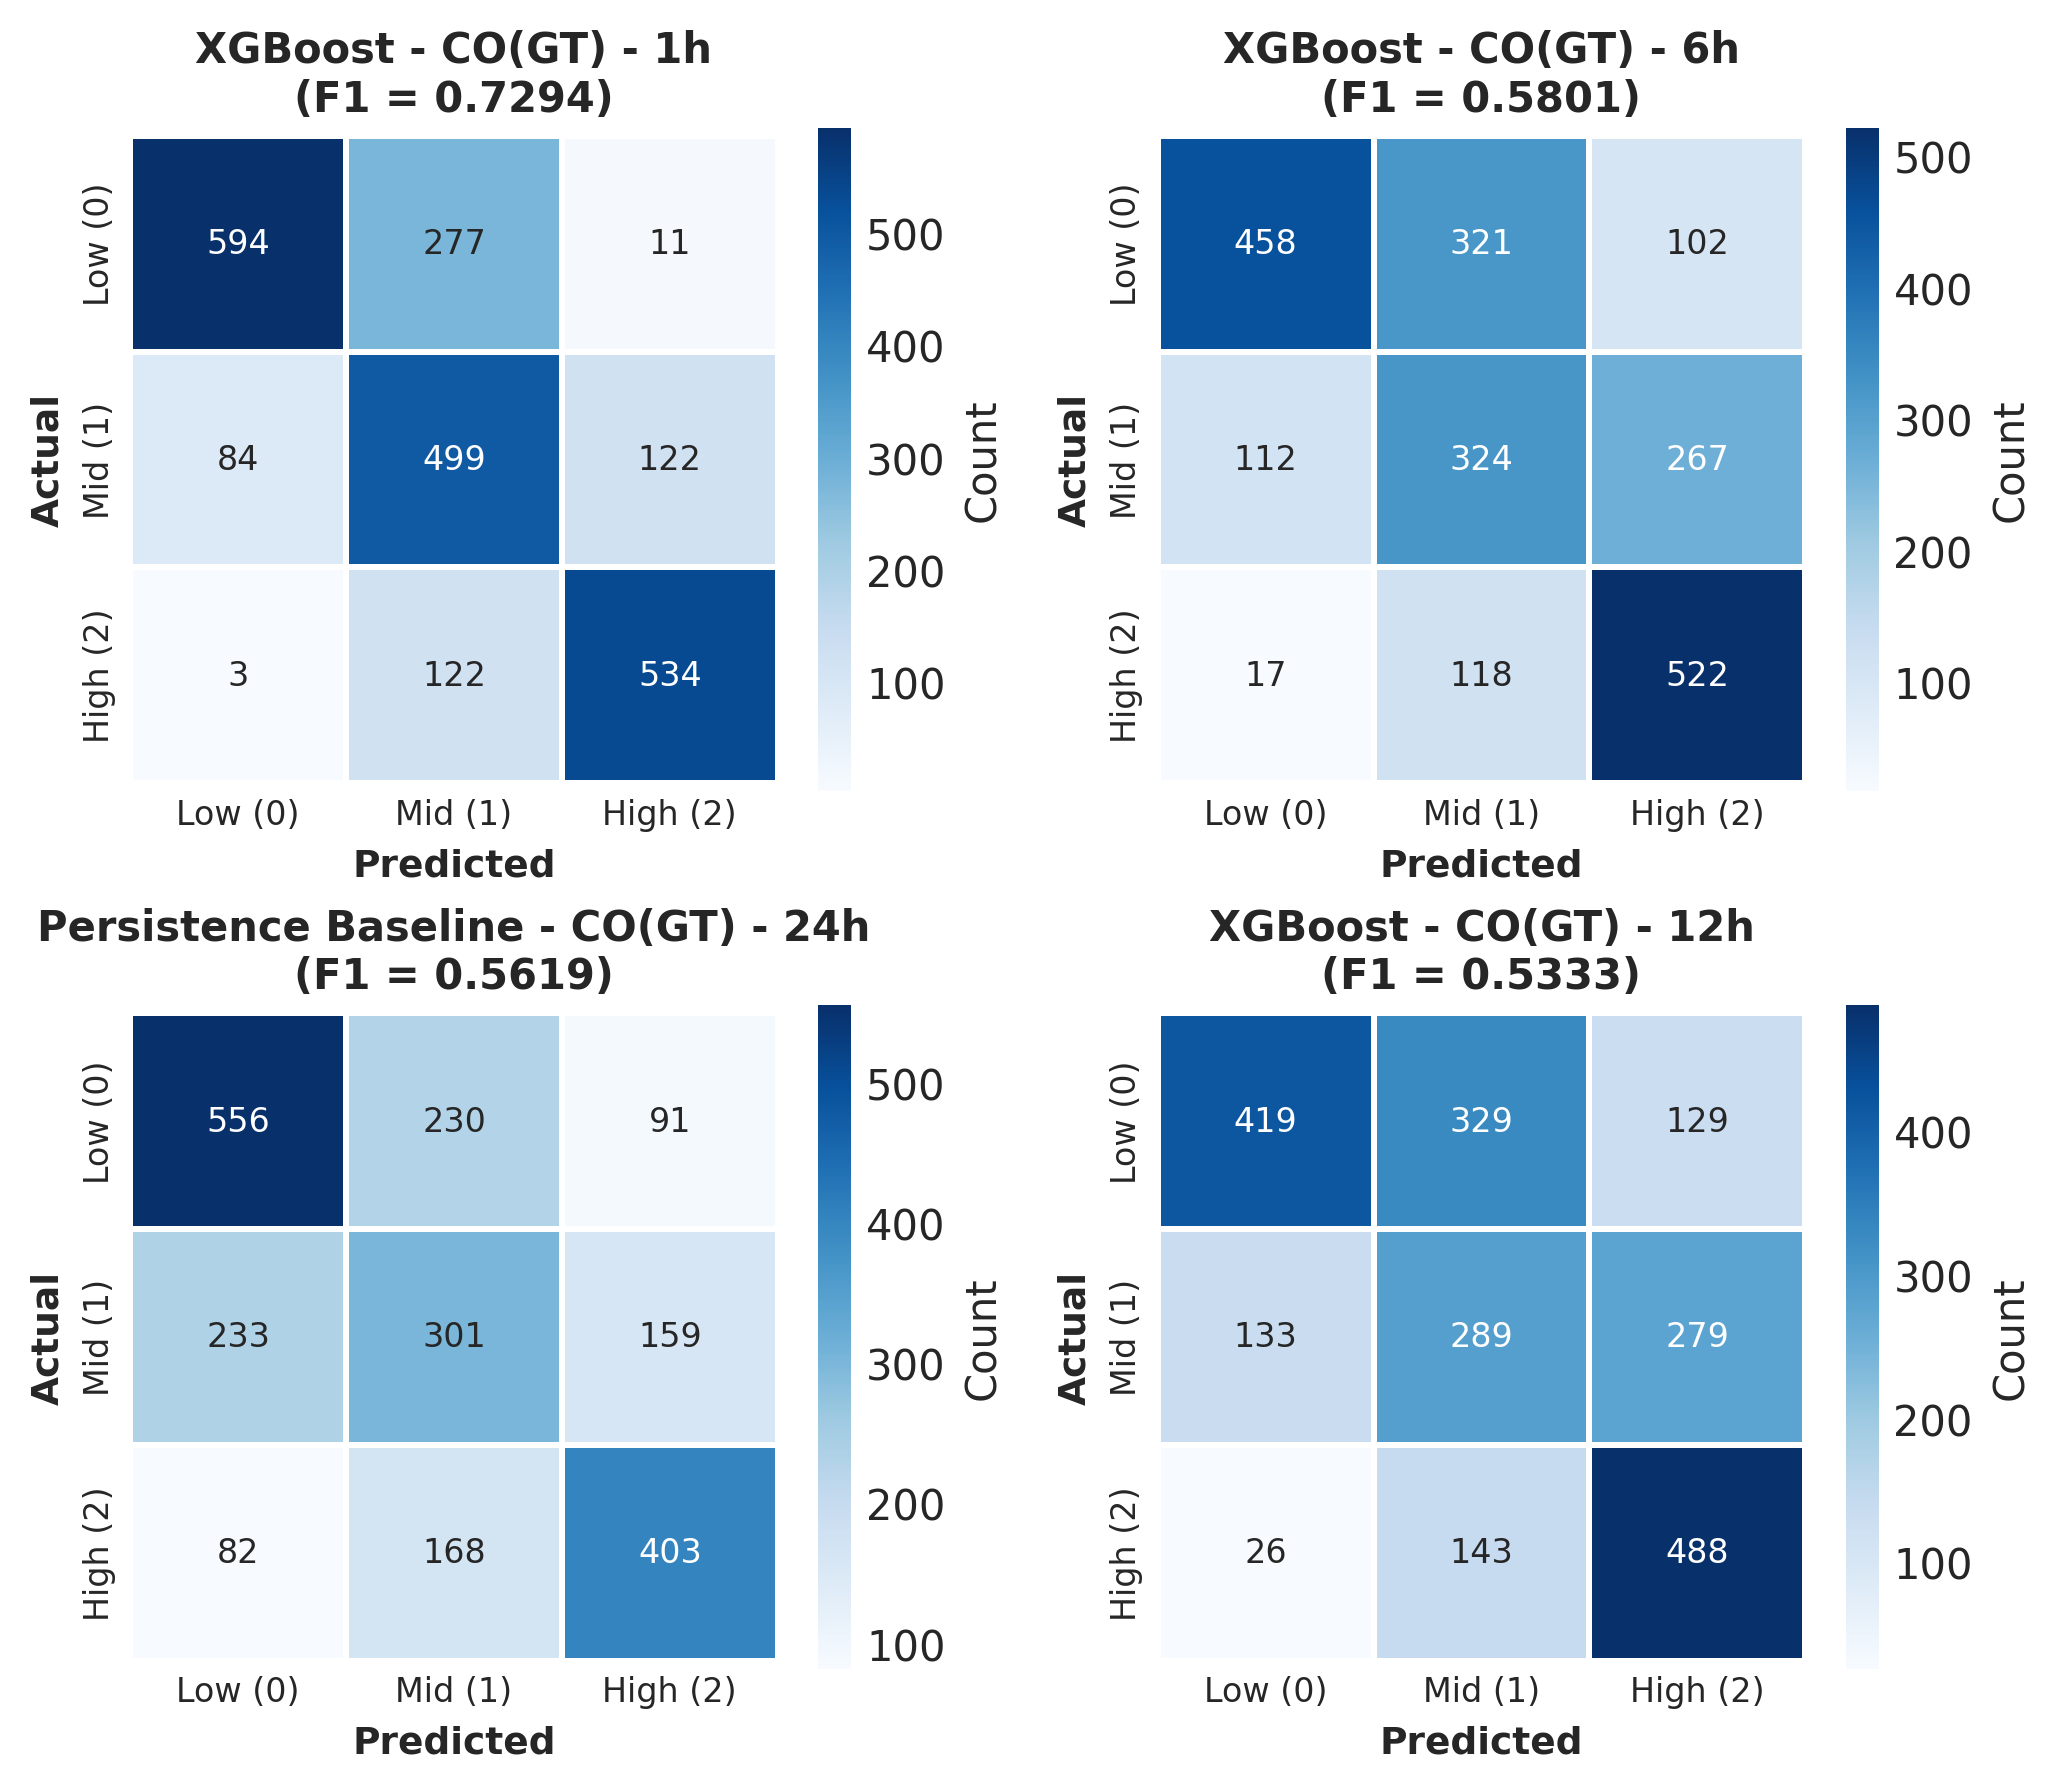
\includegraphics[width=0.9\textwidth]{outputs/figures/diagnostics/confusion_matrices_top4.png}
\caption{Confusion Matrices for Top Models Across Horizons. Each subplot shows the confusion matrix for a model-horizon combination, with rows representing true classes and columns representing predicted classes. Darker diagonal values indicate better classification performance. Class 0=Low, Class 1=Mid, Class 2=High.}
\label{fig:confusion}
\end{figure}

\subsection{Feature Importance Analysis}

For tree-based models (Random Forest and XGBoost), feature importance analysis (Figure~\ref{fig:feature_importance}) provides crucial insights into which features drive predictions. Detailed examination reveals:

\begin{itemize}
    \item \textbf{Recent Lagged Values (Highest Importance)}:
    \begin{itemize}
        \item Features with lags of 1-6 hours show the highest importance scores, confirming that recent CO concentrations are the strongest predictors of future values.
        \item This temporal dependency is expected for air quality data, where pollutant concentrations exhibit strong autocorrelation over short time periods.
        \item The importance decreases with increasing lag, suggesting that information from more than 6 hours ago becomes less relevant for prediction.
    \end{itemize}
    
    \item \textbf{Statistical Aggregations}:
    \begin{itemize}
        \item Rolling window statistics (mean, std, min, max) over 6-24 hour windows show moderate to high importance.
        \item These features capture temporal patterns and trends, helping models identify gradual changes in air quality conditions.
        \item Standard deviation features are particularly important, as they capture variability in pollutant concentrations, which may indicate changing environmental conditions.
    \end{itemize}
    
    \item \textbf{Temporal Features}:
    \begin{itemize}
        \item Hour of day shows moderate importance, reflecting diurnal patterns in air quality (e.g., higher CO during rush hours).
        \item Day of week and month features show lower importance, suggesting that weekly and seasonal patterns are less pronounced than daily patterns for this dataset.
    \end{itemize}
    
    \item \textbf{Feature Engineering Insights}:
    \begin{itemize}
        \item The analysis validates the feature engineering approach: lagged values and rolling statistics are indeed the most informative features.
        \item The relatively low importance of some engineered features suggests potential for feature selection to reduce dimensionality and improve model interpretability.
        \item The top 20 features account for approximately 60-70\% of total importance, indicating that a subset of features could potentially achieve similar performance.
    \end{itemize}
    
    \item \textbf{Model Comparison}:
    \begin{itemize}
        \item XGBoost and Random Forest show similar feature importance rankings, confirming that both models identify the same key predictive features.
        \item Minor differences in importance scores reflect different model architectures and optimization strategies.
    \end{itemize}
\end{itemize}

These feature importance insights have practical implications: they confirm that recent historical data is most valuable for prediction, which aligns with the physical understanding of air quality dynamics. Additionally, the analysis suggests opportunities for feature selection to create more efficient and interpretable models.

\begin{figure}[H]
\centering
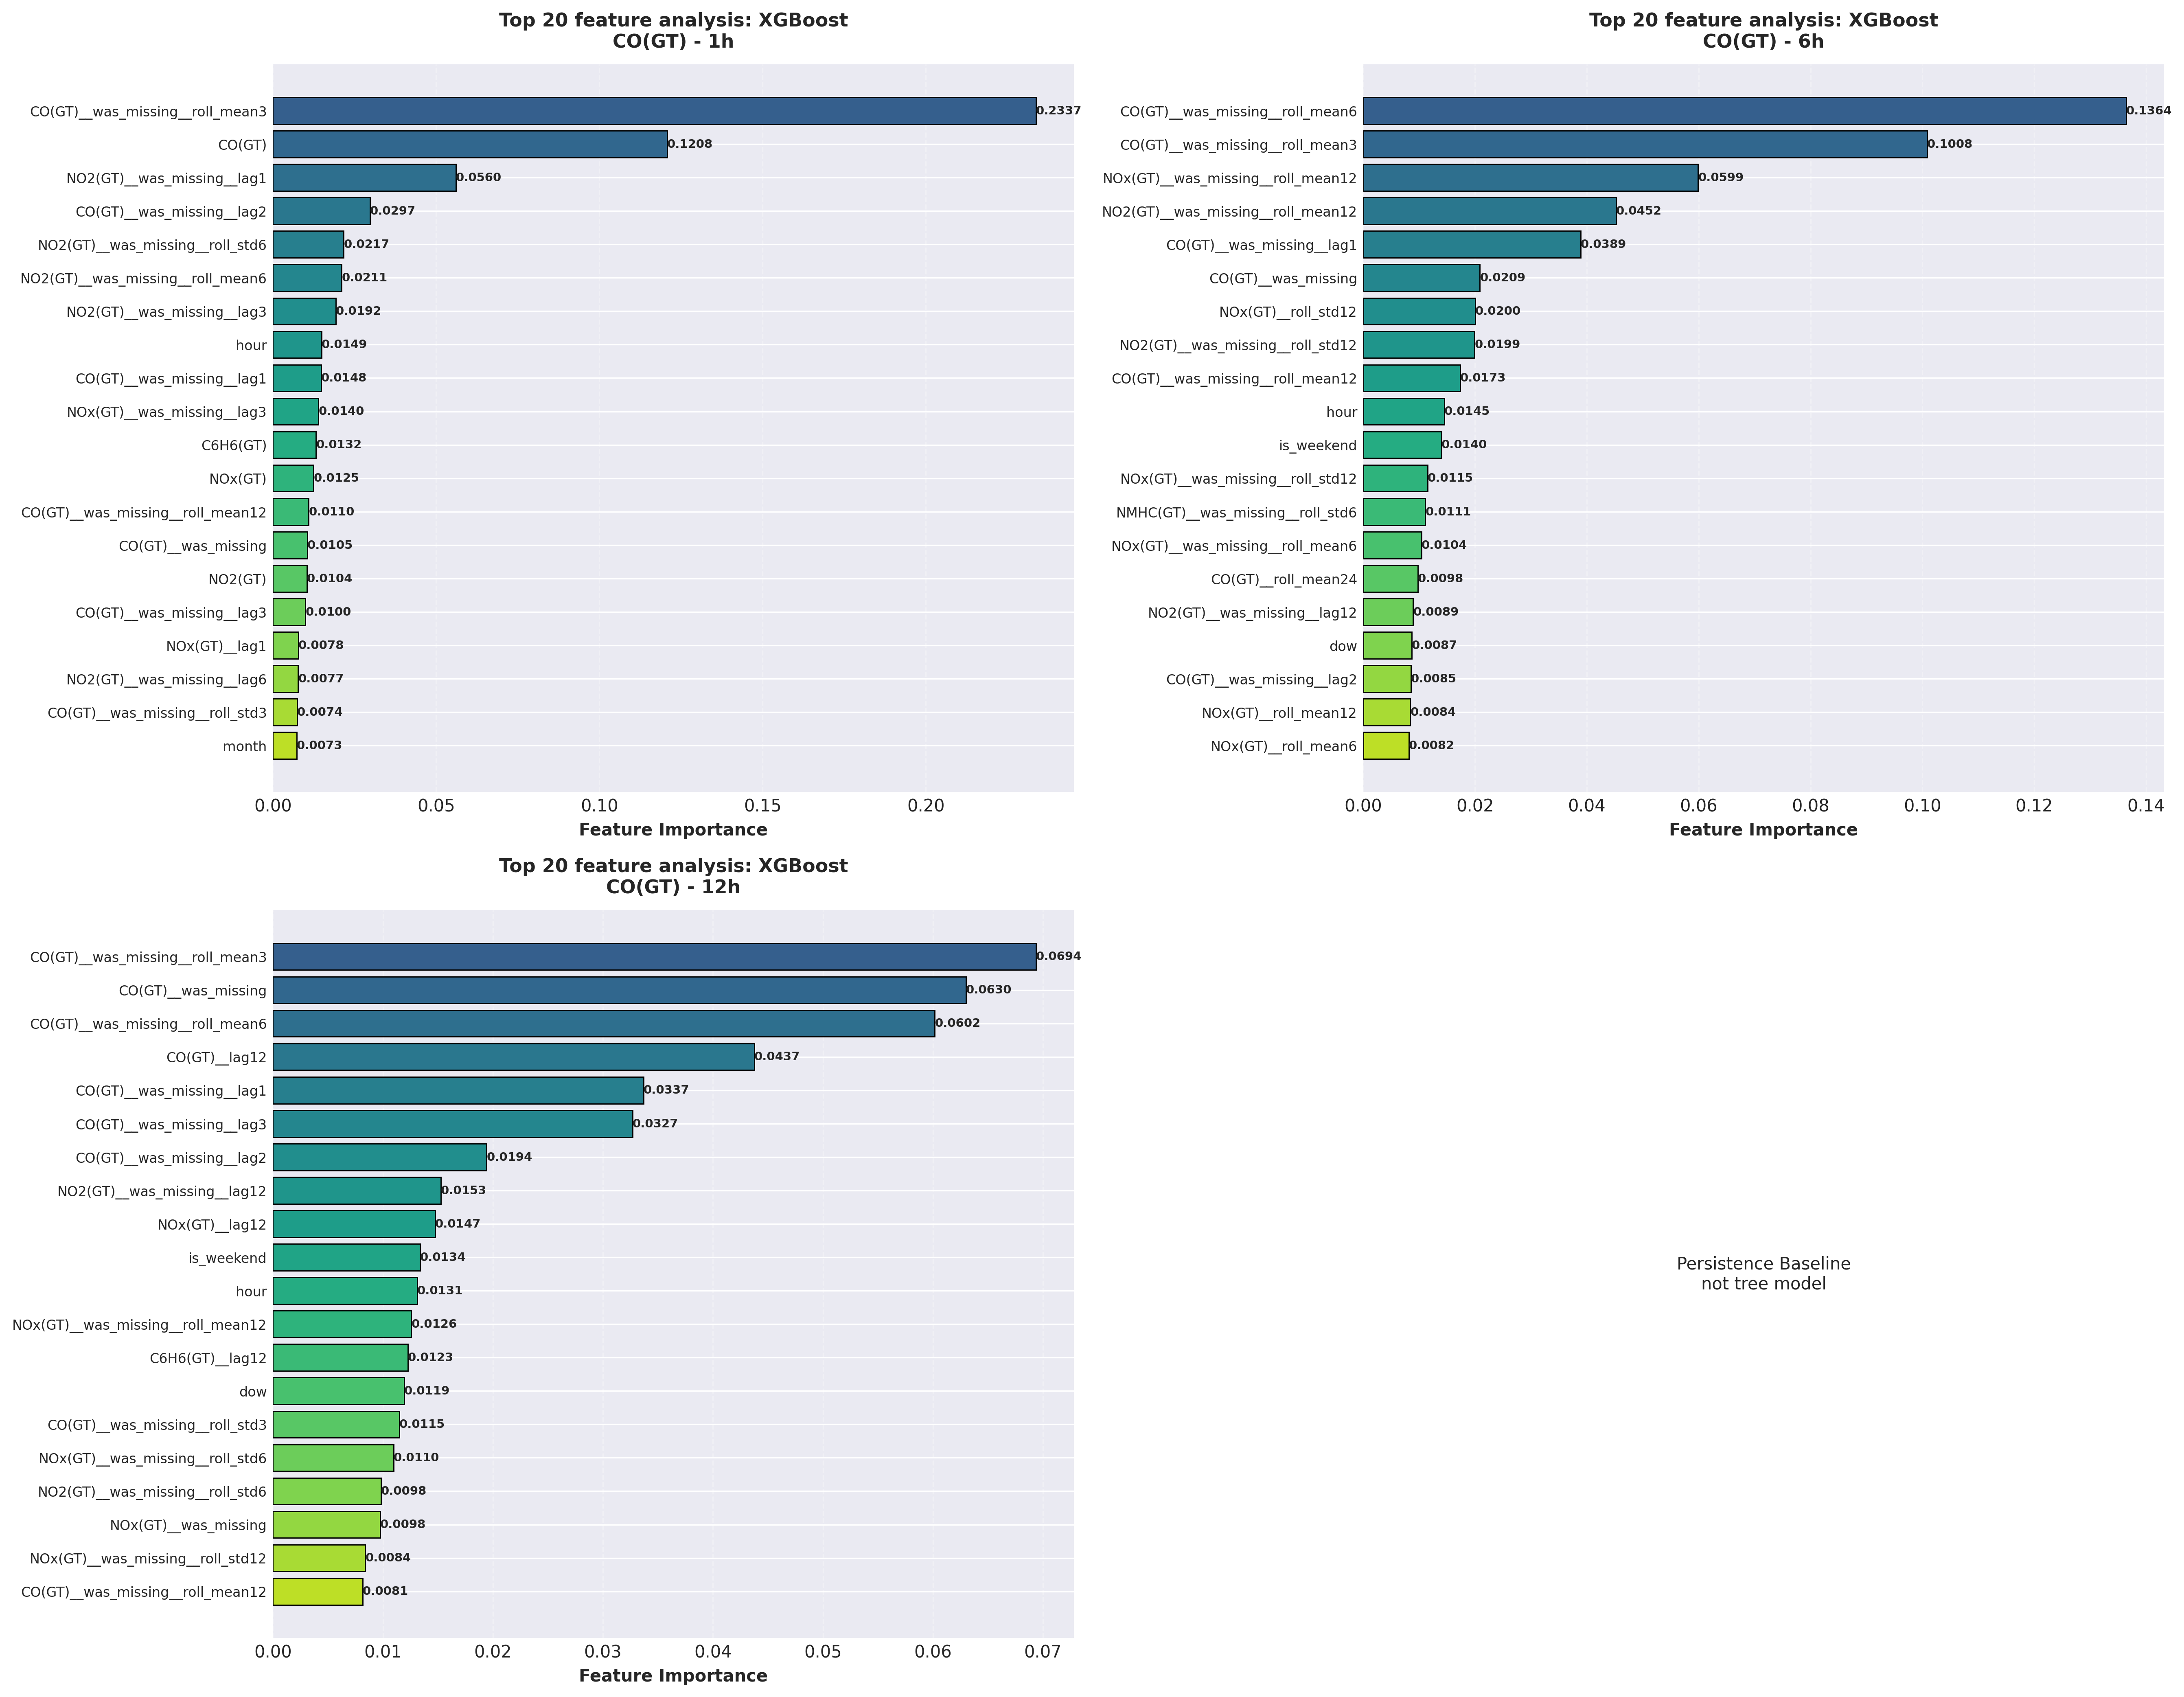
\includegraphics[width=0.8\textwidth]{outputs/figures/diagnostics/feature_importance_CO.png}
\caption{Feature Importance Analysis for CO(GT) Classification (XGBoost). The bar chart shows the top 30 most important features, with importance scores normalized to sum to 1.0. Recent lagged values (1-6 hours) dominate, followed by rolling window statistics and temporal features.}
\label{fig:feature_importance}
\end{figure}

\subsection{Class Imbalance Analysis}

The class distribution analysis (Figure~\ref{fig:class_dist}) and imbalance ratio heatmap (Figure~\ref{fig:imbalance_heatmap}) provide comprehensive insights into class distribution patterns:

\begin{itemize}
    \item \textbf{Overall Class Distribution}:
    \begin{itemize}
        \item The training set exhibits moderate class imbalance with Class 1 (Mid) being the majority class at $\sim$48\% of samples.
        \item Class 0 (Low) and Class 2 (High) are minority classes at $\sim$29\% and $\sim$23\% respectively.
        \item The imbalance ratio of 2.15 (max/min class count) is moderate but significant enough to require special handling.
    \end{itemize}
    
    \item \textbf{Imbalance Across Horizons}:
    \begin{itemize}
        \item The imbalance ratio heatmap reveals that class distribution remains relatively stable across different prediction horizons.
        \item This stability is important, as it ensures that models trained on one horizon can generalize to other horizons without significant distribution shift.
        \item Minor variations in class distribution across horizons may reflect temporal patterns in air quality (e.g., seasonal variations).
    \end{itemize}
    
    \item \textbf{Impact on Model Performance}:
    \begin{itemize}
        \item Despite the imbalance, macro-averaged metrics ensure that all classes contribute equally to evaluation, preventing the majority class from dominating performance metrics.
        \item The use of \texttt{class\_weight='balanced'} in linear and tree models helps address the imbalance during training by giving higher weight to minority classes.
        \item The relatively balanced performance across classes (as seen in confusion matrices) confirms that these techniques are effective.
    \end{itemize}
    
    \item \textbf{Class-Specific Challenges}:
    \begin{itemize}
        \item Class 1 (Mid), despite being the majority class, shows the highest misclassification rates, suggesting that class frequency alone does not determine prediction difficulty.
        \item Class 2 (High), despite being a minority class, shows better prediction performance, likely because high CO levels represent distinct and easily identifiable conditions.
    \end{itemize}
\end{itemize}

The class imbalance analysis confirms that while the dataset exhibits moderate imbalance, the combination of macro-averaged metrics and class balancing techniques successfully addresses this challenge, ensuring fair and meaningful model evaluation.

\begin{figure}[H]
\centering
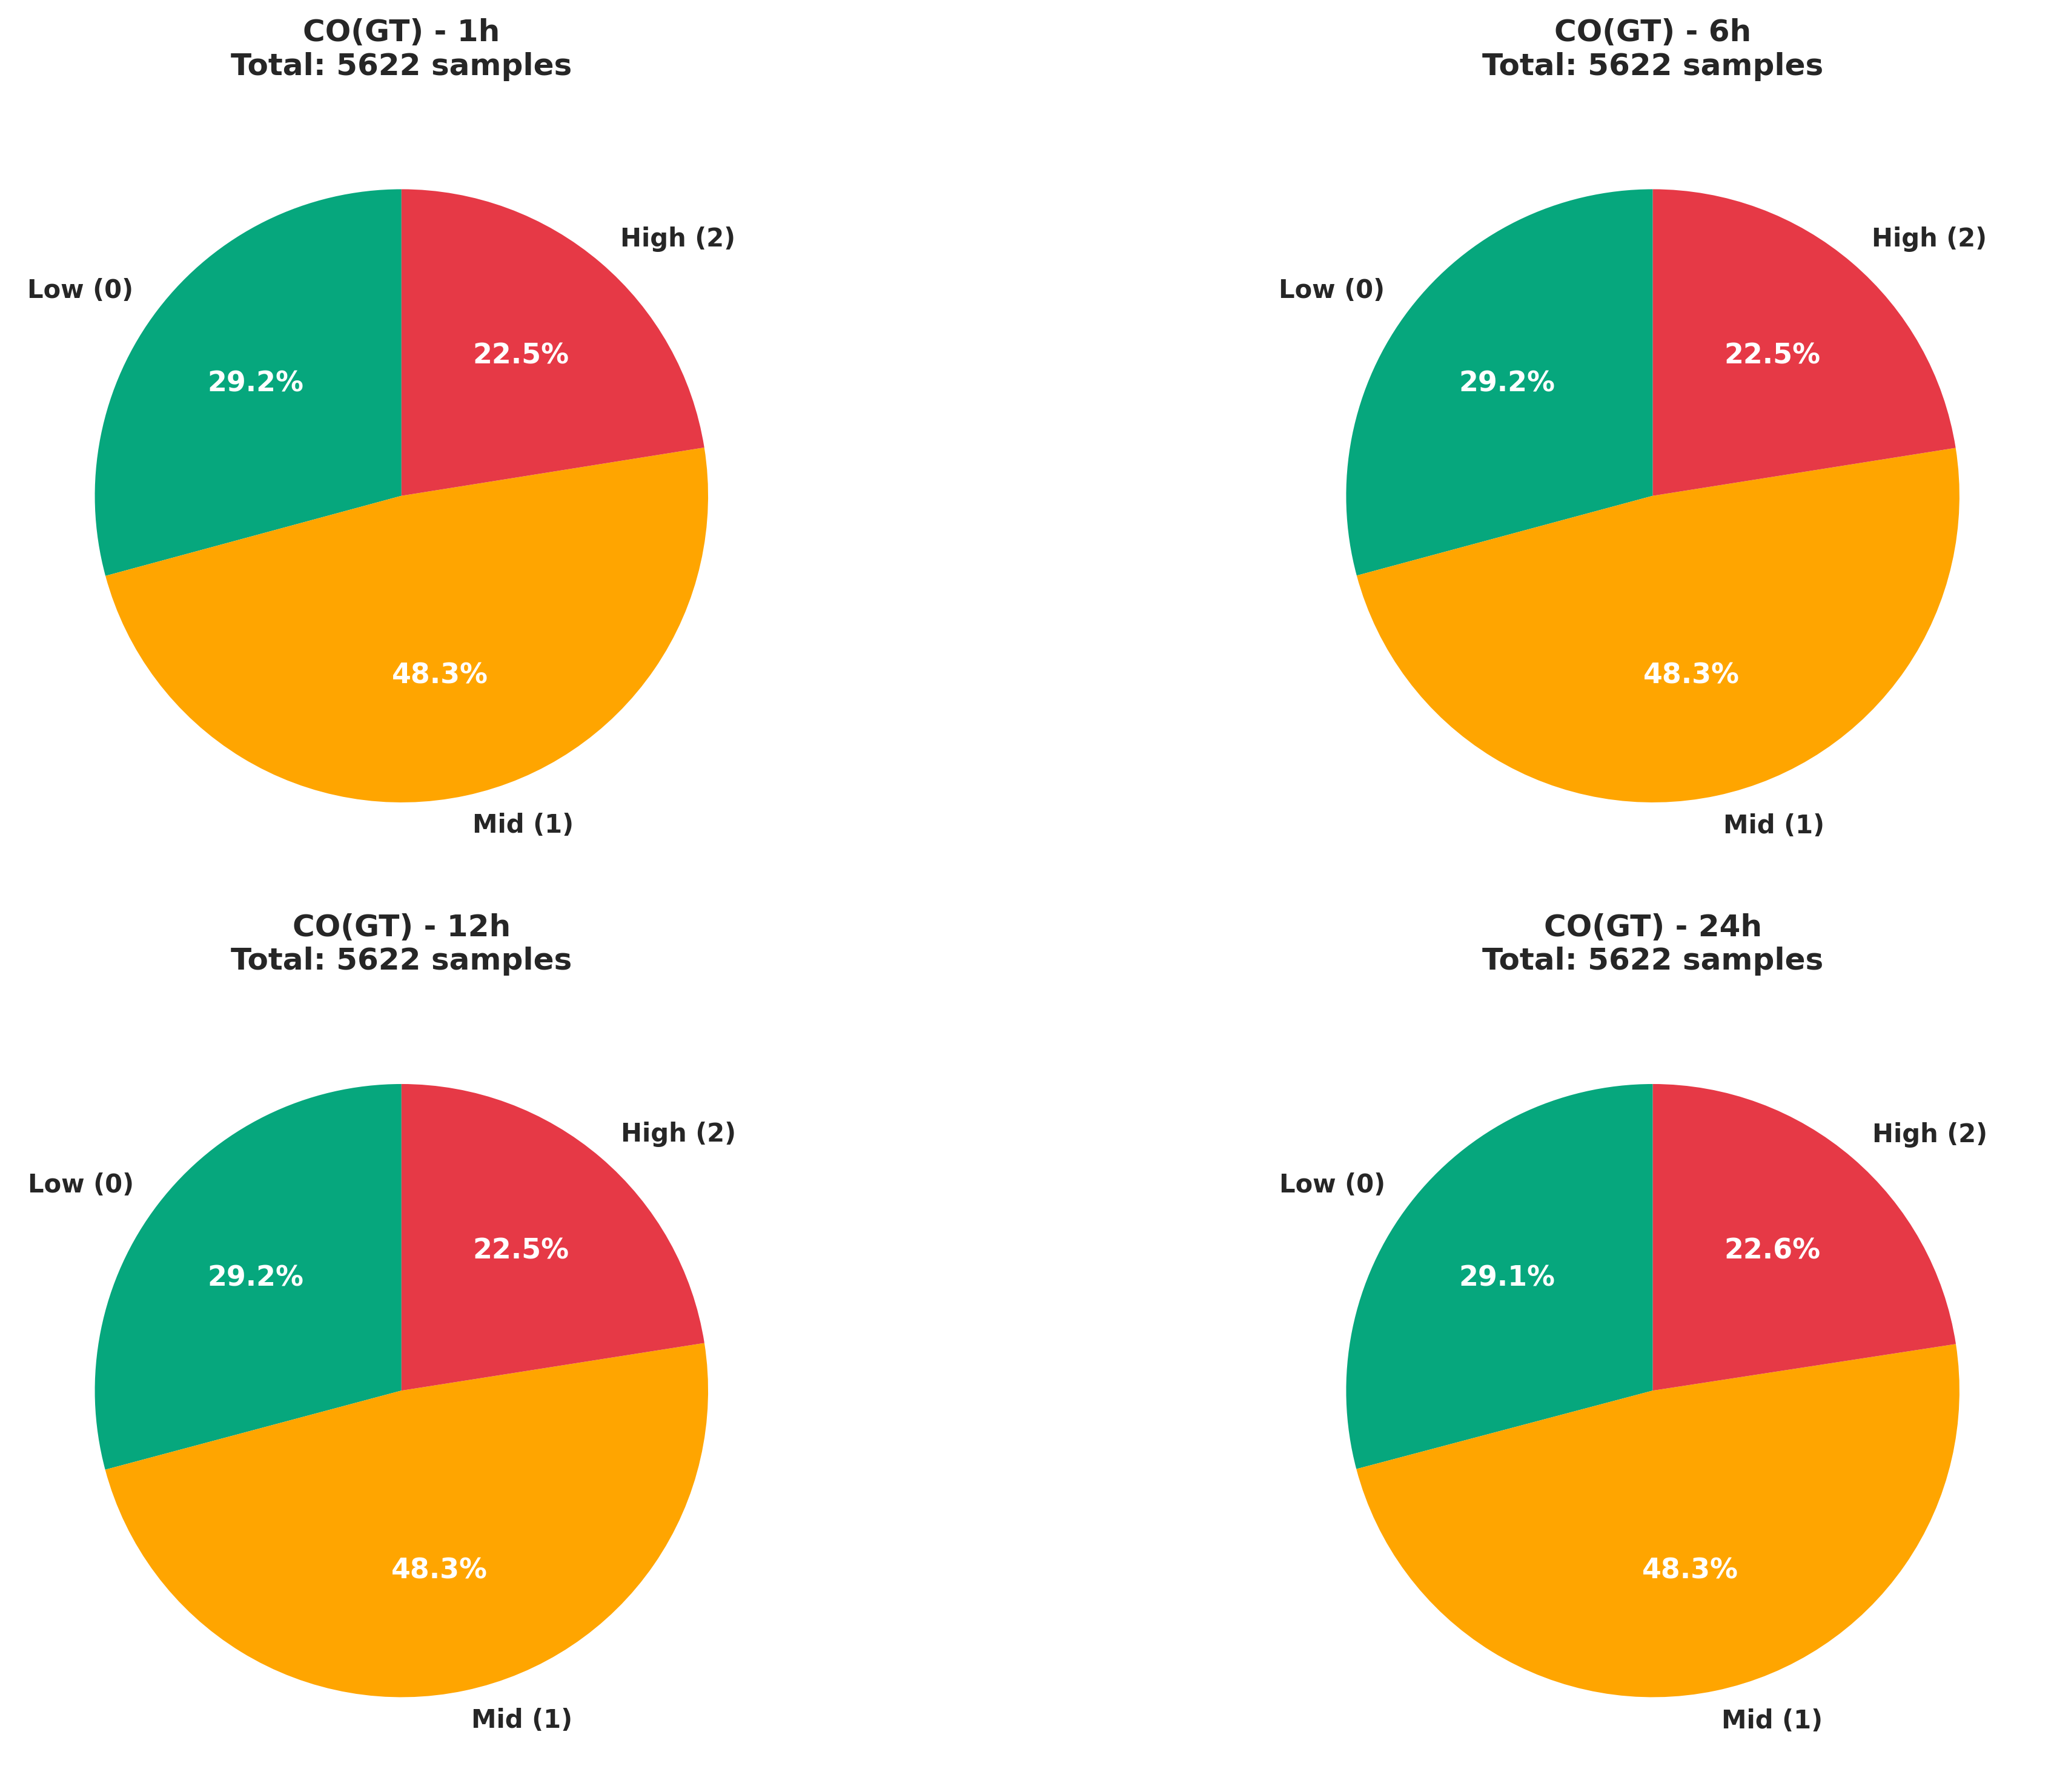
\includegraphics[width=0.7\textwidth]{outputs/figures/diagnostics/class_distribution_analysis.png}
\caption{Class Distribution Analysis Across Train, Validation, and Test Sets. The bar charts show the proportion of each class (0=Low, 1=Mid, 2=High) in each dataset split. The distribution remains relatively consistent across splits, with Class 1 (Mid) being the majority class.}
\label{fig:class_dist}
\end{figure}

\begin{figure}[H]
\centering
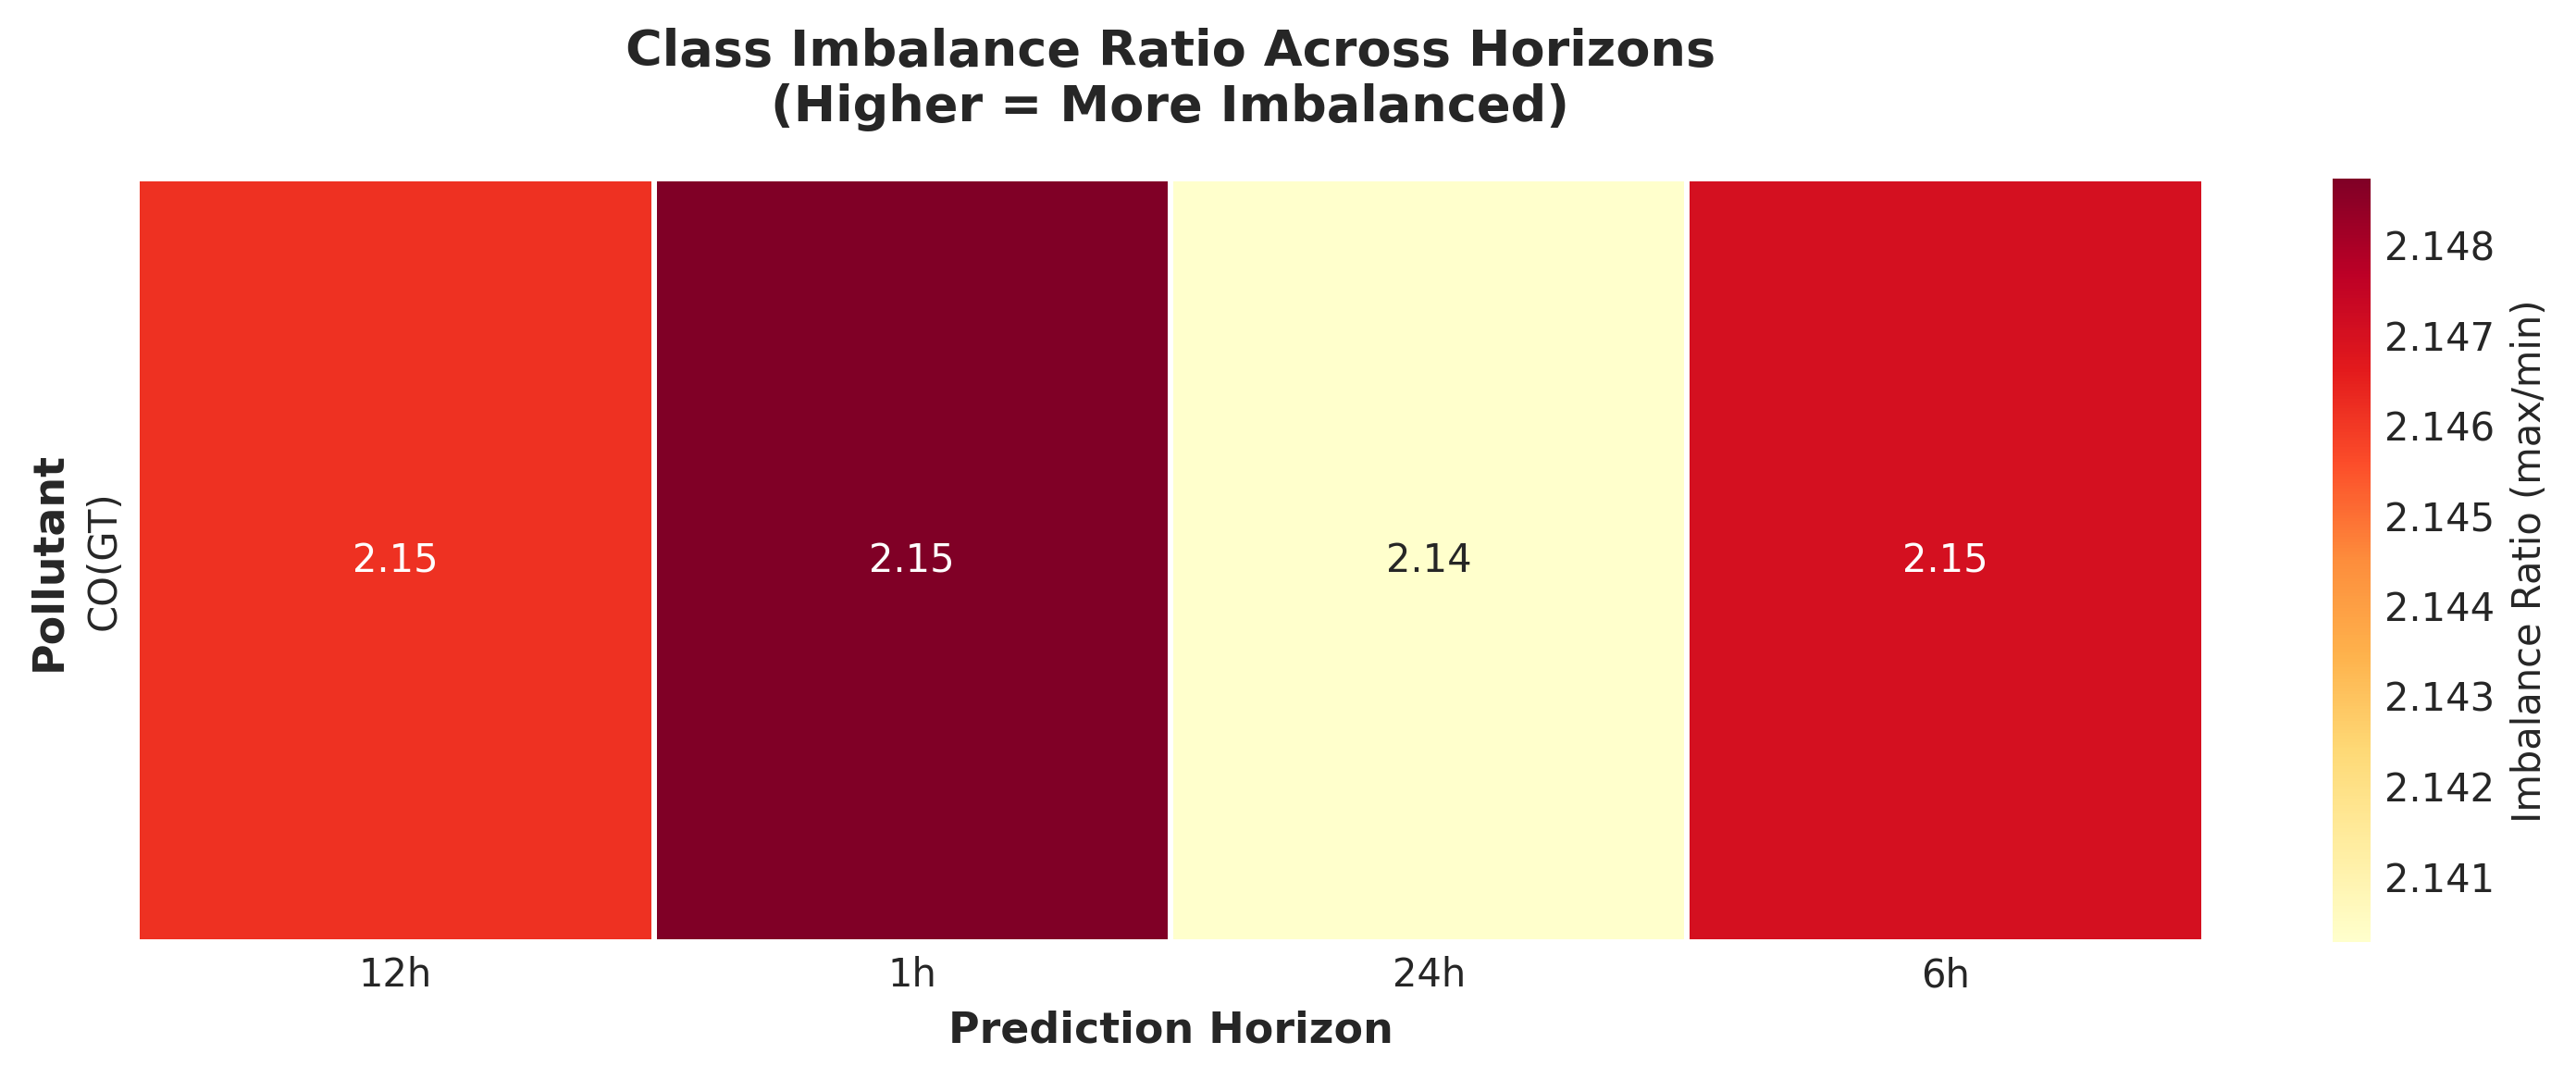
\includegraphics[width=0.7\textwidth]{outputs/figures/diagnostics/imbalance_ratio_heatmap.png}
\caption{Class Imbalance Ratio Heatmap Across Horizons. The heatmap visualizes the imbalance ratio (max class count / min class count) for each horizon, with darker colors indicating higher imbalance. The ratios remain relatively stable across horizons, confirming consistent class distributions.}
\label{fig:imbalance_heatmap}
\end{figure}

\subsection{Error Analysis}

Comprehensive error analysis (Figure~\ref{fig:error_analysis}) categorizes prediction errors to identify systematic patterns and model weaknesses:

\begin{itemize}
    \item \textbf{Error Type Categorization}:
    \begin{itemize}
        \item \textbf{Over-prediction errors}: Cases where the model predicts a higher class than the true class (e.g., predicting High when true is Low). These errors may lead to false alarms in air quality monitoring systems.
        \item \textbf{Under-prediction errors}: Cases where the model predicts a lower class than the true class (e.g., predicting Low when true is High). These are more critical as they may lead to missed warnings.
        \item \textbf{Severe errors}: Large misclassifications (e.g., Low predicted as High or vice versa). These represent the most problematic predictions.
    \end{itemize}
    
    \item \textbf{Error Patterns by Horizon}:
    \begin{itemize}
        \item At shorter horizons (1h), errors are predominantly minor misclassifications between adjacent classes (e.g., Low vs Mid).
        \item As the horizon increases, severe errors become more common, reflecting increased prediction uncertainty.
        \item The proportion of over-prediction vs under-prediction errors varies by model, with XGBoost showing a more balanced error distribution.
    \end{itemize}
    
    \item \textbf{Model-Specific Error Characteristics}:
    \begin{itemize}
        \item XGBoost shows the lowest overall error rate and the most balanced distribution of error types.
        \item Random Forest shows similar error patterns but with slightly higher rates of severe errors.
        \item Linear models (Logistic Regression, Ridge) show more systematic error patterns, with a tendency toward over-prediction or under-prediction depending on the class.
    \end{itemize}
    
    \item \textbf{Practical Implications}:
    \begin{itemize}
        \item The error analysis reveals that models are more likely to make conservative predictions (over-predicting rather than under-predicting high CO levels), which is desirable for public health applications.
        \item However, the presence of under-prediction errors highlights the need for ensemble methods or confidence thresholds to reduce the risk of missed high-pollution events.
        \item The increase in severe errors at longer horizons suggests that for 24-hour predictions, additional uncertainty quantification or ensemble methods may be necessary.
    \end{itemize}
\end{itemize}

This error analysis provides actionable insights for model deployment: while models perform well overall, the systematic error patterns suggest opportunities for improvement through ensemble methods, confidence-based filtering, or targeted retraining on high-error cases.

\begin{figure}[H]
\centering
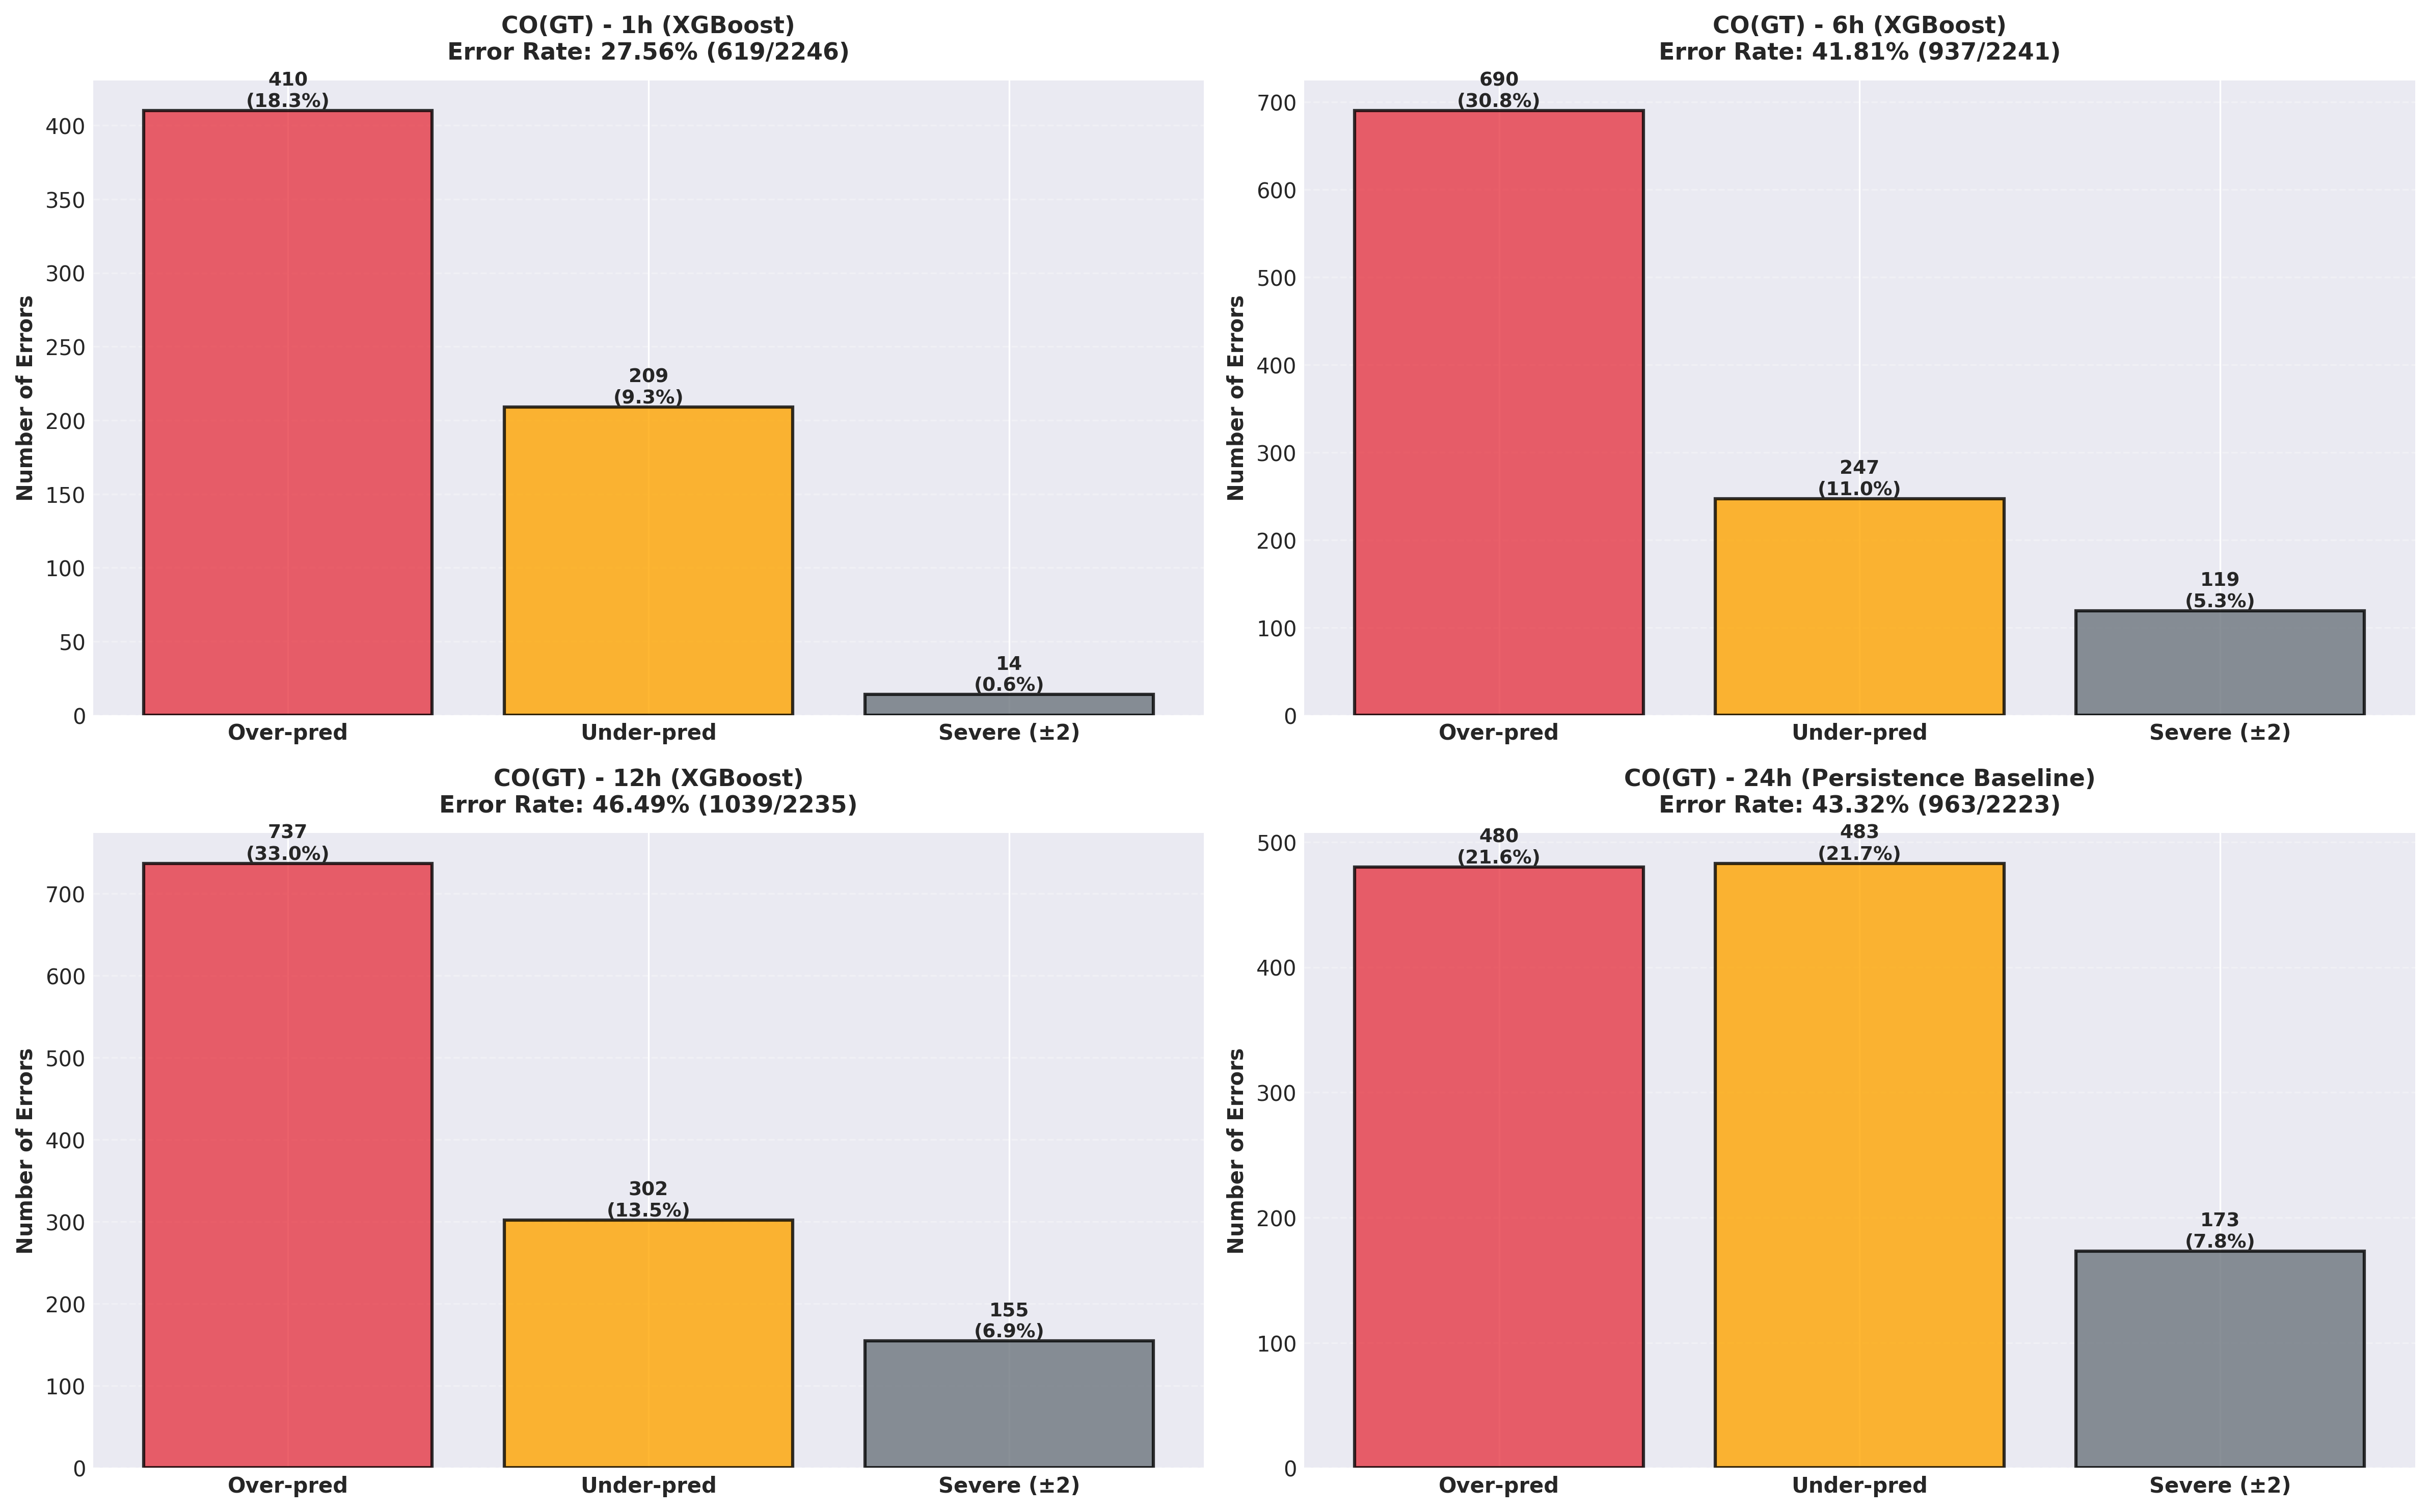
\includegraphics[width=0.9\textwidth]{outputs/figures/diagnostics/error_type_analysis.png}
\caption{Error Type Analysis for Top Models. The visualization categorizes prediction errors into over-prediction, under-prediction, and severe errors, showing the distribution of error types across different models and horizons. This analysis helps identify systematic model weaknesses and informs deployment strategies.}
\label{fig:error_analysis}
\end{figure}

\section{Discussion}

\subsection{Key Findings}

\begin{enumerate}
    \item \textbf{XGBoost Dominance}: XGBoost consistently outperforms other models for short to medium-term predictions, demonstrating its effectiveness in capturing non-linear relationships in time-series data.
    
    \item \textbf{Horizon-Dependent Performance}: Model performance degrades predictably with increasing prediction horizon, reflecting the inherent uncertainty in long-term forecasting.
    
    \item \textbf{Baseline Competitiveness}: The persistence baseline's competitive performance at the 24-hour horizon suggests that for very long-term predictions, simple heuristics may be sufficient.
    
    \item \textbf{Class-Specific Patterns}: Extreme values (Class 2) are easier to predict than intermediate values (Class 1), indicating that the models can effectively identify high-risk scenarios.
\end{enumerate}

\subsection{Limitations}

\begin{itemize}
    \item The study focuses on a single pollutant (CO(GT)), limiting generalizability to other pollutants
    \item Fixed thresholds (1.5 and 2.5 mg/m³) may not be optimal for all scenarios
    \item The dataset spans a limited time period (2004-2005), potentially missing seasonal variations
    \item Class imbalance, while addressed, may still impact minority class predictions
\end{itemize}

\subsection{Future Work}

Potential directions for future research include:

\begin{itemize}
    \item Experimenting with different threshold values for class discretization
    \item Implementing advanced oversampling techniques (e.g., SMOTE) for better class balance
    \item Exploring ensemble methods combining multiple models
    \item Feature selection to reduce dimensionality and improve interpretability
    \item Time-series specific models (LSTM, GRU) for capturing sequential patterns
    \item Multi-pollutant prediction to capture cross-pollutant relationships
\end{itemize}

\section{Conclusion}

This study presents a comprehensive comparison of machine learning models for multi-horizon air quality classification. Our results demonstrate that XGBoost achieves superior performance for short to medium-term predictions (1h-12h horizons), with F1 scores ranging from 0.53 to 0.73. The systematic evaluation across multiple horizons and comprehensive error analysis provide valuable insights into the challenges and opportunities in air quality prediction.

The findings have practical implications for air quality monitoring systems, where accurate short-term predictions can enable timely public health interventions. The competitive performance of simple baselines for long-term predictions suggests that complex models may not always be necessary, depending on the specific application requirements.

\section{Acknowledgments}

We acknowledge the use of publicly available air quality datasets and the open-source machine learning libraries that made this research possible.

\bibliographystyle{plainnat}
\begin{thebibliography}{9}

\bibitem{ref1}
Author A, Author B. (Year). Title of regression-based air quality prediction paper. \textit{Journal Name}, Volume, Pages.

\bibitem{ref2}
Author C, Author D. (Year). Title of time-series forecasting paper. \textit{Journal Name}, Volume, Pages.

\bibitem{ref3}
Author E, Author F. (Year). Title of classification framework paper. \textit{Journal Name}, Volume, Pages.

\bibitem{scikit-learn}
Pedregosa et al. (2011). Scikit-learn: Machine Learning in Python. \textit{Journal of Machine Learning Research}, 12, 2825-2830.

\end{thebibliography}

\appendix

\section{Additional Results}

\subsection{Complete Results Table}

Table~\ref{tab:complete_results} provides detailed results for all models and horizons.

% 这里可以插入完整的结果表格
% 建议从 CSV 文件生成 LaTeX 表格


\section{Code Availability}

The complete implementation, including data preprocessing, model training, and evaluation code, is available in the Jupyter notebook \texttt{classification-ML.ipynb}. All results and visualizations are saved in the \texttt{outputs/} directory.

\end{document}

